% !TEX TS-program = xelatex
% !Mode:: "TeX:UTF-8"

\documentclass[bachelor, english]{uestcthesis}

% math 
\usepackage{bm}	% bold math

% math font
%\usepackage{mathptmx}	% times font
\usepackage{standalone}


% def, theorems, etc
\theoremstyle{plain}
\newtheorem{thm}{Theorem}[chapter] % reset theorem numbering for each chapter
\newtheorem{lemma}{Lemma}[chapter]

\theoremstyle{definition}
\newtheorem{defn}{Definition}[chapter] 
\newtheorem{exmp}{Example}[chapter] 

% math shorthands
\newcommand{\argmax}{\operatornamewithlimits{argmax}}
\newcommand{\argmin}{\operatornamewithlimits{argmin}}
\newcommand{\Var}{\operatornamewithlimits{Var}}
\newcommand{\E}{\operatornamewithlimits{E}}

% here it goes

\begin{document}
% !TEX TS-program = latex
% !TEX root = Thesis_Guo2013.tex

\chapter{Introduction}
The tasks of estimation, inference and prediction, as an essential constituent of human activities, have been embraced by researchers in computer science, especially in the field of \textit{Artificial Intelligence (AI)}. 
To solve these tasks, researchers make use of both the mathematical formalism and the computational power realized by modern hardware and programming tools. 
Unfortunately, due to the continuing influences of the early pioneers and their paradigms, for a while AI scientists equated reasoning with ``rational'' deduction; and tried to come up with if-then-else rules for various prediction tasks \cite{ravikumar2007}.

However, in the recent several decades, a noticeable paradigm shift occurred in the field of AI. 
More modern influences such as quantum physics and statistics made many appreciate the use of probabilistic machinery, not just for modeling uncertainty but for making efficient estimations and predictions possible at all. From then on, scientists in AI growingly rely on probability theory and statistics as the formalism for seeking both theoretical insights into problems and justifications for methods and algorithms \cite{russell2010book}. 

Even a sub-field called \textit{machine learning} emerged from the general stream of AI. 
While AI emphasizes the study and design of intelligent agents, including  a group of interacting agents, as the central topic, machine learning is more specific in both its objective and methodology. Machine learning is concerned with discovering patterns, making inferences and predictions from \textit{data} and it shares the same formal framework with probability and statistics, which is also the paradigm adopted in this thesis.

In a probabilistic perspective, a central and fundamental task would be the characterization of the distribution of random variables, including the marginal of each variable and the interdependence among them. Ideally, the fullest characterization would be given by writing down the joint distribution of the all the variables involved. Yet, among others, due to the usually unknown or partially observable mechanism underlying real-world data or the ``curse of dimensionality'' coming with a large number of variables, one has to assume less accurate but more compact forms of representation of the joint distribution, such as log-linear models, Markov random fields and Bayesian networks \cite{bishop2006prml}.

Once we have data and the estimated distribution of the variables in concern, it would be desirable to know the properties of the distribution, for the purpose of developing learning algorithms that utilizes these properties or summarizing the large-volume data into a straightforward, human-perceptible form. Among others, moments are the simplest measures for quantitatively characterizing the shape of distributions. For example, if we have the data tracking a noisy signal and find that the signal follows a Gaussian distribution, we would then like to know the mean and standard deviation of the noise, for the first measure tells us around what value the signal fluctuates and the second informs us the amplitude of the fluctuation. 

Moments are also important in their role connecting data and the population. In a statistical point of view, the data collected are considered as a part out of an infinite sea of data that are not fully observed, which are called \textit{statistical population}. On one hand, we use the data to estimate the distribution of population; on the other hand, we assume that future, unobserved data and the data available now are sampled from \textit{the same} population so that our model can be \textit{generalized} to unknown or future cases. 

Specifically, a moment simultaneously corresponds to a sample moment and a population moment, where the former characterizes how data in hands are distributed and the latter characterizes how the population are distributed. A sample moment is computed by performing simple algebraic operations on data, e.g. the arithmetic mean is the sum of all observation of a variable divided by the number of observations; a population moment is obtained by getting the mathematical expectation of a polynomial function of the random variable, which is usually done in the form of integral, e.g. the population mean is the mathematical expectation of the random variable itself.  

The relation between the sample moments and the corresponding population moments are known when the population moments converge --- a sample moment converges to the corresponding population moment by probability when the size of samples extends to infinity. Therefore, in the convergent case, we can use the sample moments calculated with a large sample to estimate the shape of the population distribution. In the traditional statistical literature, because the distributions encountered (e.g. Gaussian, exponential) are usually exponentially bounded in tails, population moments of all positive orders would naturally converge. As a result, the convergence of moments are often assumed without explicit mention and the relation between the two kinds moments is largely ``taken for granted'' in practice.

However, such a naive notion towards moments and the general assumption of moments being convergent should be brought to serious examination when dealing with today's ever diversified data. A distinctive exception to the moment-convergent assumption is a family of distributions called \textit{heavy-dutyed distributions}, where the density functions in this family have heavier tails than the exponential distributions \cite{asmussen2003applied}, rendering their moments with orders higher than a threshold divergent. Heavy-tailed distributions ``appear'' more common than before with the development of information technology, as data can now be collected and assembled from an unprecedented large scale, e.g. data collected from the whole Internet, from millions of online users and from hundreds of countries around the world. For example, \textit{power-law distributions}, as a member of the heavy-tail family, are found in the distributions for the degrees of the Internet, the population of cities around the world and the citations of papers in academic communities \cite{Clauset2009}. 

When dealing with data exhibiting these distributions, it is possible that a certain moment of interest is divergent. Then, the sample moment do not converge when the sample size grows bigger, but instead grows with the size. In this thesis, I will first seek to clarify the underlying mechanism beneath the divergence of moments and the relation between sample and population moments in this case. Then I will propose a method that systematically analyzes the asymptotic behavior of sample moments under convergence as the sample size extends to infinity. Furthermore, I will discuss the application of this method in analyzing heavy-tailed distributions, especially power-law distributions. Before addressing the method for analyzing divergent moments, I would like to outline some key concepts involved as background materials for this work.

\section{Random variables and probability distributions}
\subsection{Random variables}
Probability theory deals with the analysis of the likelihood of random events defined over a sample space $ \Omega $ . For example, consider rolling a single fair die, where we denote the value rolled as $ X $ and the sample space as $ \Omega $. The sample space of a single roll can be defined as $\Omega = \{1, 2, 3, 4, 5, 6\}$ and the possible random events are subsets of $ \Omega $ . For example, we can consider the event that $ X=4 $  is rolled as well as the event that an even value is rolled. If an event is a single element of the sample space $ X \in \Omega $  then we refer to the event as an atomic event. The event that $ X=4 $  is rolled is an example of an atomic event.

When dealing with random events we are often interested in numerical descriptions of the events and not just the probability of the event occurring. In order to handle this we can assign numerical descriptions of events to what are referred to as random variables. For example, $ X $ is a random variable in rolling one fair die. And supposing that we roll two fair dice, we also can define a random variable $ Y $  to take on the numerical result of the sum of the dice. 

\begin{defn}
A random variable $ X $  defined over a sample space $ \Omega $  is a function $ X: \Omega \rightarrow \mathbb{R} $ that maps an event $ X \in \Omega $  to a real value.
\end{defn}

Random variables that only take on values from a countable set (such as the integers) are referred to as discrete random variables. The random variable defined as the sum of the roll of two fair dice is an example. Random variables that take on values from an uncountable set (such as the reals) are referred to as continuous random variables. For example, the arrival time for the next car in a highway intersection is a continuous random variable.

\subsection{Probability distributions}
In analyzing random variables we are often interested in the probability that a random variable takes on certain values. To formally describe the different probabilities of a random variable taking on various values we define a probability distribution.

\begin{defn}
A probability distribution $ P $ defined on random variable $ X $  over a sample space $ \Omega $  is a mapping from events $ \alpha \in \Omega $  to real values on the interval $ [0,1] $  such that $ P(\alpha) \geq 0 $  and $ P(\Omega)=1 $ .
\end{defn}


\section{Moment}
In statistics, a moment is, loosely speaking, a quantitative measure of the shape of a distribution. For example, mean, as the simplest moment, measures around what value the distribution is centered around; and variance, as the second central moment, measures how much the distribution disperses around the mean; while some moments of higher orders describe other aspects of a distribution such as how the distribution is skewed from its mean, or peaked. While moments can be extended to multivariate distributions, such as \textit{image moments} that are used in 2-D image processing \cite{hu1962visual}, we will focus on univariate distributions due to the scope of this thesis. 

\subsection{Expectation and Riemann-Stieltjes integral}
A population moment with regard to a probability distribution is formally defined as the \textit{mathematical expectation} of a polynomial function of the random variable. And a rigorous, unified treatment of expectation relies \textit{Riemann-Stieltjes integral}, which is a generalized form for the \textit{Riemann integral}. Therefore, we will first briefly outline these concepts before moments are introduced.

Whereas the usual Riemann integral of a real-valued function $ g(x) $ with regard to the variable $ x $ on a range $ [a,b] $ is usually denoted by $ \int_a^b g(x) dx $, a Riemann-Stieltjes integral for $ x $  involves two functions. The Riemann-Stieltjes integral for $ g(x) $ with regard to another real function $ F(x) $ is denoted by $ \int_a^b g(x)dF(x) $. It is well-known that $ \int_a^b g(x) dx $ can be interpreted as the area under $ g(x) $ with $ a \leq x \leq b $. So what does Riemann-Stieltjes integral mean? In fact, $ \int_a^b g(t) dF(t) $ (the variable is changed for convenience) can still interpreted as the area under a curve. Let us imagine $ t $ as a parameter and we now track the point $ t $ moving from $ a $ to $ b $, meanwhile drawing the curve $ (x,y)=(F(t), g(t)) $. Then the integral is simply the area under the curve, as a sum of rectangles each resulted by a every tiny move of $ t $. 

Now let us turn to a more formal definition of $ \int_a^b g(x)dF(x) $. First the range $ [a,b] $ is partitioned into $ n $ intervals with  $ a=x_0 < x_1 < \cdots < x_{n-1} < x_n=b$. Then we tag each small interval $ [x_i, x_{i+1}] $ with a representative number $ c_i $, with $ c_i \in [x_i, x_{i+1}] $. Next, 
we write down the sum of the area of small rectangles as 
\begin{equation}
S = \sum_{i=0}^{n-1} g(c_i) (F(x_{i+1})-F(x_i)).
\end{equation}
The integral can obtained by taking the limit of $ S $ while ``densifying'' the partition. The density can be measured by a \textit{mesh} of the partition, and here we just take the maximum length of the interval $ \Delta = \max_{0 \leq i \leq n-1} (x_{i+1}-x_{i})$ as the mesh. As the mesh $ \Delta \rightarrow 0 $, the partition is continually densified and the sum would converge to a limit, if it exists, which is defined to be the Riemann-Stieltjes integral. Hence, we outline the following definition. 

\begin{defn}
If there is some $ A \in \mathbb{R} $, such that for any $ \epsilon > 0 $, there exists $ \delta > 0 $ so that any $ S = \sum_{i=0}^{n-1} g(c_i) (F(x_{i+1})-F(x_i)) $ with the mesh of partition $ \Delta < \delta  $ satisfies $ |S-A|< \epsilon $, then the Riemann-Stieltjes integral $ \int_a^b g(x) dF(x) $ exists and we define $ \int_a^b g(x) dF(x) \triangleq A $.  
\end{defn}

Now we turn to the definition for mathematical expectation. For a discrete random variable $ X $, which takes values $ x_1, x_2, \cdots, x_n $ with probabilities $ p_1, p_2, \cdots, p_m $, then the expectation of $ X $ is defend to be the weighted sum, i.e.
\begin{equation}
\E[X] = \sum_{i=1}^n x_i p_i. 
\end{equation}
For a continuous random variable $ X $ with a well-defined PDF $ f(x) $, then the expectation is yield with a Riemann integral, i.e.
\begin{equation}
\E[X] = \int_{-\infty}^{+\infty} x f(x) dx.
\end{equation}
It seems that expectation needs to be treated differently for discrete and continuous variables when the Riemann-Stieltjes integral comes to the rescue. 

\begin{defn}
Given $ X $ is a random variable with its cumulative distribution function (CDF) $ F(X) $, then its expectation value is defined to be 
\begin{equation}
\E[X] = \int_{-\infty}^{+\infty} x dF(x),
\end{equation}
regardless of $ X $ being discrete or continuous. 
\end{defn}
Similarly, the expectation of the random variable $ g(X) $ as a function of $ X $ is given by
\begin{equation}
\E [g(X)] = \int_{-\infty}^{+\infty} g(x) dF(x).
\end{equation}

\subsection{Definition of moment}
Every moment is defined with its ``double identity'' --- a population moment and sample moment. Both of them are quantitative measures for the shape of the distributions, but the former is for describing the shape of the ``empirical distribution'' (the distribution for samples), i.e. the CDF constructed from data, while the latter is for characterizing the distribution of population, where a well-defined, closed-form distribution function is usually assumed. When the sample size is small, the two distributions may be different and the two moments may also differ noticeably in their values; but when the sample size grows big, the empirical distribution  will converge to that of the population by the \textit{Strong Law of Large Numbers}, and the two moments will be identical in the limit. 

But the sample moment and its corresponding population moment are different in their calculation. Without explicitly getting the CDF for the empirical distribution, one can directly calculate sample moments by performing simple algebraic operations (addition, multiplication and division) on data. But the calculation of population moment is analytic, rather than algebraic. The population distribution is usually given (or assumed to be) as a analytic function and its population moments, if exist, can be acquired by integrating a polynomial function with regard to the PDF. These two moments are also different in their existence: a population moment does not exist if the integral diverges; a sample moment $ always $ exists because it is a algebraic outcome computed from data.

\subsubsection{Population moment}
A \textit{population moment} can be understood as a particular distance measure defined by the distribution with a point as its reference. When there is no ambiguity, we also refer to \textit{population moment} as \textit{moment} for short. 
\begin{defn}
Given a univariate PDF $ f(x) $ for the distribution of a random variable $ X $ , the $ n $-th moment taken about a point $ c $ is defined as $ \mu_n(c) = \int_{-\infty}^{+\infty} (x-c)^n f(x) dx $ \footnote{When addressing the definition of moments, we assume $ X $ is a continuous variable for simplicity. The discrete case can be similarly defined by replacing the integral with sum.} , if the integral converges.   
\end{defn}

The reference point $ c $ is often chosen to be $ 0 $ or the mean. When $ c=0 $, the moment is called \textit{raw moment}.

\begin{defn}
The $ n $-th raw moment is defined as $ \mu'_n = \mu_n(0) $, where $ \mu_n(c) $ is the moment taken about $ c $. 
\end{defn}
    
$ \mu'_1 $ is simply the $ mean $ of the distribution, and we have $ \mu'_0=1 $ due to the normalization of a distribution. For moments of higher orders, we are often concerned with the moment taken around the mean, which is called \textit{central moment}.

\begin{defn}
The $ n $-th central moment is defined as $ \mu_n = \mu_n(\mu'_1) $, where $ \mu_n(c) $ is the moment taken about $ c $ and $ \mu'_1 $ is the mean.    
\end{defn}

It shall be noted the following definitions rely on the condition that the integral for defining the moment is convergent, which is always the case for distributions with exponentially bounded tails, but not necessarily true for other distributions. 

\subsubsection{Sample moment}
\textit{Sample moments} are the same metrics as population moments, except that they are defined by the \textit{empirical distributions} of data, rather than the assumed the distribution function. Sample moments can be computed by performing simple algebraic operations on data and every moment $ \mu_n(c) $ has one sample counterpart $ m_n(c) $.

\begin{defn}
Given a sample $ \{x_1, x_2, \cdots, x_N\} $ with size $ N $, the $ n $-th sample moment with reference to $ c $ is defined as $ m_n(c) = \frac{1}{N} \sum_{i=1}^N (x_i-c)^n $.
\end{defn}

As samples are always finite numbers, a sample moment \textit{always} exists regardless of existence of the corresponding population moment. \textit{Sample raw moments} can be defined in a parallel fashion.

\begin{defn}
Given a sample $ \{x_1, x_2, \cdots, x_N\} $ with size $ N $, the $ n $-th sample raw moment is defined as $ m'_n = m_n(0) $.  
\end{defn}

Sample moments can be used as estimators for the corresponding population moments, which we would discuss later.

\subsection{Moments in common uses}
We now describe some population moments that are widely used in statistics for characterizing the shape of distributions. 

\subsubsection{Mean}
Mean is the first raw moment $ \mu'_1 $, which gives the value around which the distribution is centralized around.

\begin{figure}[!h]
\begin{center}
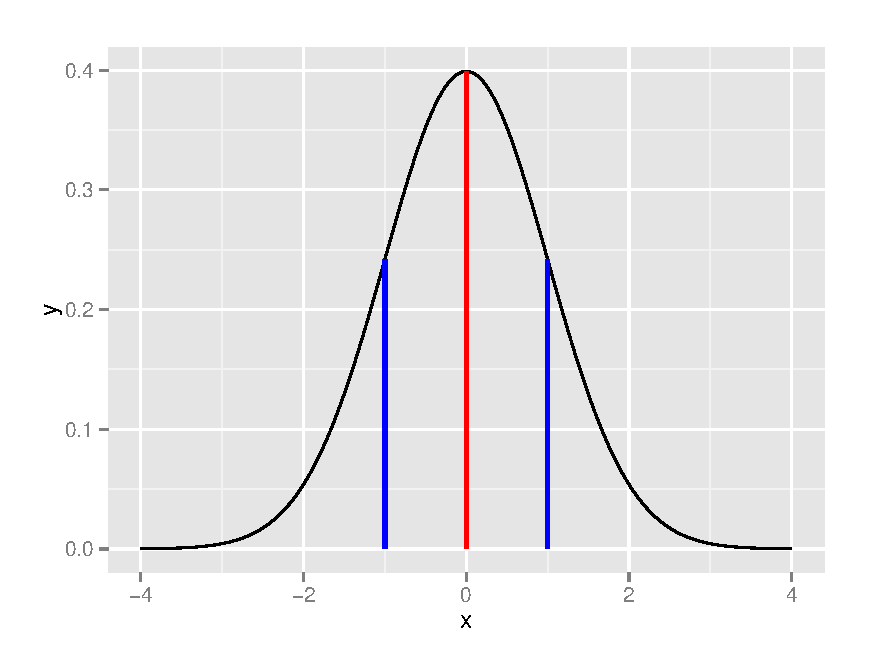
\includegraphics[width=0.8\textwidth]{figures/ch1_gaussian.eps}
\caption{The PDF for a standard Gaussian distribution, where the red vertical marks the value of $ \mu_1' $ and two blue lines mark $ \pm \sigma$. }
\label{fig:ch1_meanvar}
\end{center}
\end{figure}

\subsubsection{Variance}
Variance is the second central moment $ \mu_2 $, which describes how far the distribution spreads out around the mean. Its positive squared root $ \sigma $ is referred to as the \textit{standard deviation}. For the special case of Gaussian distributions, the distribution can be fully characterized by the mean and the variance, as shown in Fig. \ref{fig:ch1_meanvar}.

\subsubsection{Skewness}
The third central moment $ \mu_3 $ is a measure of the lopsidedness of the distribution; any \textit{symmetric} distribution will have a third central moment, if defined, of zero. When using higher order moments, it is a common practice to normalize the $ k $-th moment by the standard deviation to the power of $ k $.  

\begin{defn}
The $ k $-th standardized moment for a probability distribution is defined as $ \mu_k / \sigma^k $, where $ \mu_k $ is the $ k $-th central moment and $ \sigma $ is the standard deviation.
\end{defn}

In other words, the $ k $-th standardized moment is simply a \textit{normalzied} version of the $ k $-th moment with respect to the standard deviation. The power of $ k $ is used, because moments scale as $ x^k $ , meaning that $ \mu_k'(\lambda X) = \lambda^k \mu_k'(X) $:  they are homogeneous polynomials of degree $ k $ , thus the standardized moment is \textit{scale invariant}. This can also be understood as being because moments have dimension; in the above ratio defining standardized moments, the dimensions cancel, so they are dimensionless numbers.

Specifically, the \textit{standardized} third central moment $ \mu_3 / \sigma^3 $ is called the skewness, often denoted by $ \gamma_1 $, i.e.

\begin{defn}
The skewness for a random variable $ X $ is defined as $ \gamma_1 = \E[(\frac{x-\mu}{\sigma})^3] = \frac{\mu_3}{\sigma^3} $, where $ \mu $  
\end{defn}

As plotted by Fig. \ref{fig:ch1_skew}, a distribution that is skewed to the left (the tail of the distribution is heavier on the left) will have a negative skewness. A distribution that is skewed to the right (the tail of the distribution is heavier on the right), will have a positive skewness.

\begin{figure}[htbp]
\begin{center}
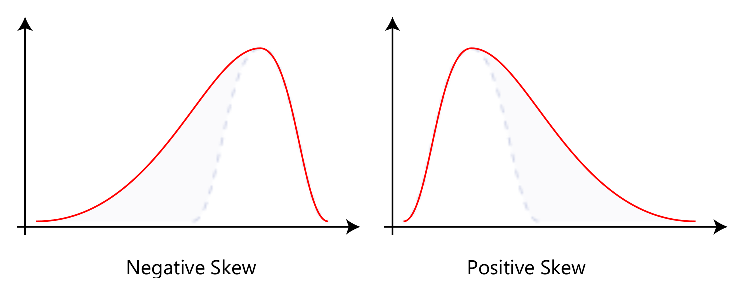
\includegraphics[width=0.8\textwidth]{figures/ch1_skew.eps}
\caption{Probabilty distributions with a negative skewness has a fatter or longer tail on the left side, and distributions with a positive skewness has a fatter or longer tail on the right side. (figure excerpted from \cite{www-wiki-skewness})}
\label{fig:ch1_skew}
\end{center}
\end{figure}

\subsubsection{Kurtosis}
The fourth central moment is a measure of whether the distribution is tall and skinny or short and squat, compared to the normal distribution of the same variance. Since it is the expectation of a fourth power, the fourth central moment, where defined, is always non-negative. 

One common measure of kurtosis, originating with Karl Pearson, is based on a scaled version of the fourth moment of the data or population, but it has been argued that this measure really measures heavy tails, and not peakedness. It is common practice to use an adjusted version of Pearson's kurtosis, the excess kurtosis, to provide a comparison of the shape of a given distribution to that of the normal distribution ($ \mu_4 $ for a normal distribution is $ 3\sigma^4 $). Fig. \ref{fig:ch1_kurtosis} shows three distributions of the same family with different values of kurtosis. 

\begin{defn}
The excess kurtosis for a random variable, if it exists, is defined as $ \gamma_2 = \mu_4 / \sigma^4 -3 $, where $ \mu_4 $ is the fourth central moment and $ \sigma $ is the standard deviation.
\end{defn}

\begin{figure}[!h]
\begin{center}
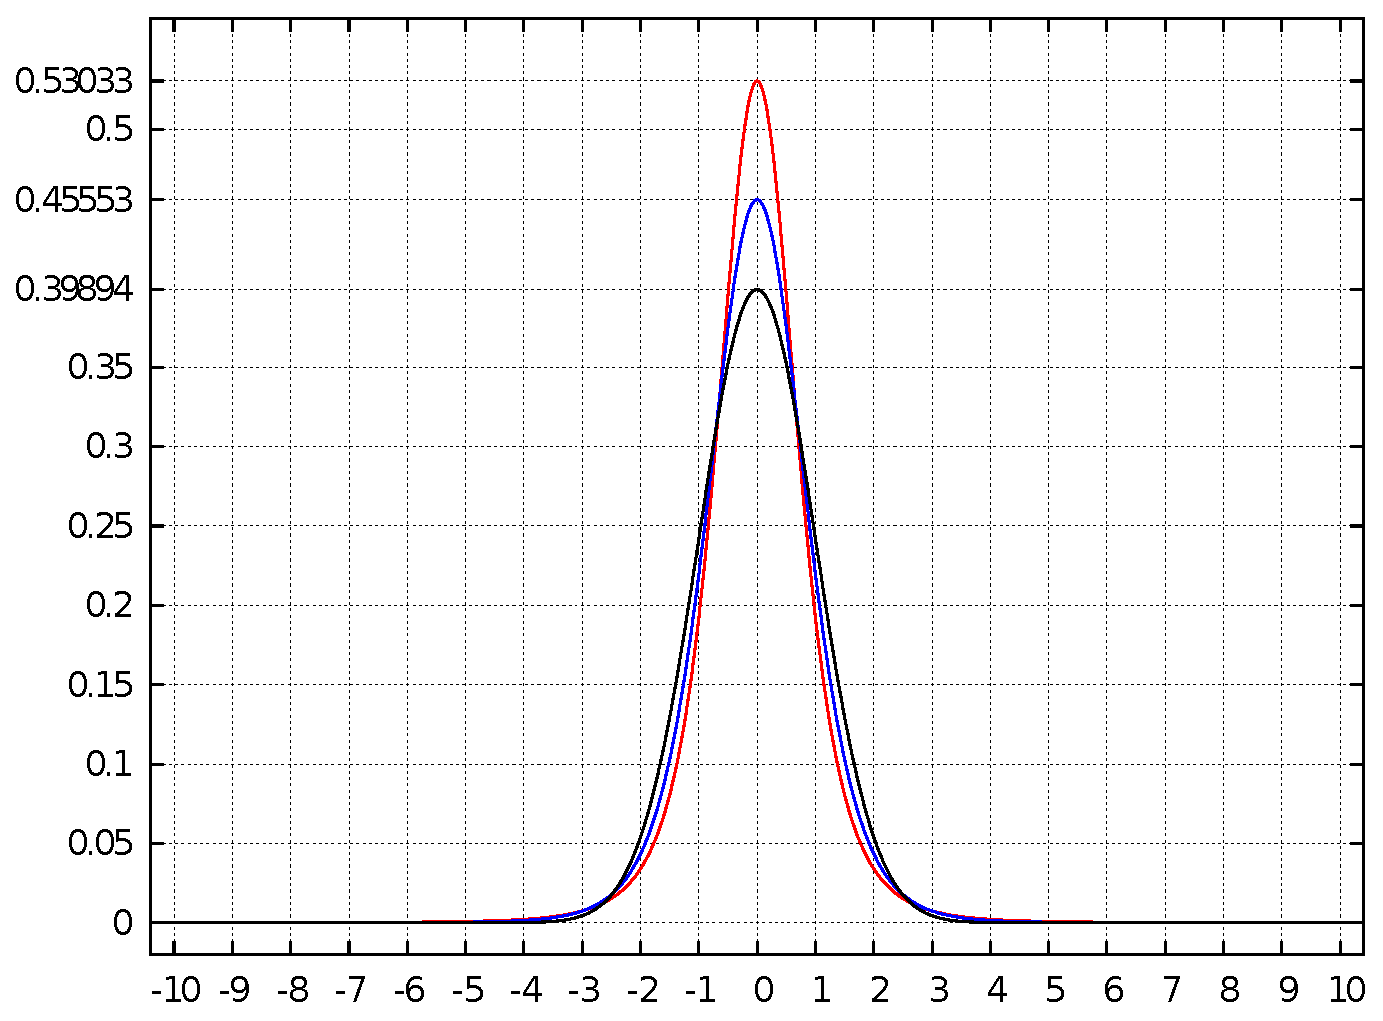
\includegraphics[width=0.7\textwidth]{figures/ch1_kurtosis.eps}
\caption{PDF for the Pearson type VII distributions with kurtosis of infinity (red), 2 (blue) and 0 (black). }
\label{fig:ch1_kurtosis}
\end{center}
\end{figure}

\subsubsection{Covariance and correlation coefficient}
\textit{Covariance} and \textit{correlation} are \textit{mixed moments} of most frequent uses. While the aforementioned moments only involve a single random variable, \textit{mixed moments} are moments of multiple random variables. 

In probability theory and statistics, covariance is a measure of how much two random variables change together. If the greater values of one variable mainly correspond with the greater values of the other variable, and the same holds for the smaller values, i.e., the variables tend to show similar behavior, the covariance is positive. In the opposite case, when the greater values of one variable mainly correspond to the smaller values of the other, i.e., the variables tend to show opposite behavior, the covariance is negative. The sign of the covariance therefore shows the tendency in the linear relationship between the variables.

\begin{defn}
The covariance between two jointly distributed real-valued random variables $ X $  and $ Y $  with finite second moments is defined as
\begin{equation}
\sigma(x,y) = \E \left [ (X-\E(X))(Y-E(Y)) \right].
\end{equation}
\end{defn}

After some algebra, covariance can be rewritten in the form as 
\begin{align}
\sigma(X,Y)
&= \operatorname{E}\left[\left(X - \operatorname{E}\left[X\right]\right) \left(Y - \operatorname{E}\left[Y\right]\right)\right] \nonumber\\
&= \operatorname{E}\left[X Y - X \operatorname{E}\left[Y\right] - \operatorname{E}\left[X\right] Y + \operatorname{E}\left[X\right] \operatorname{E}\left[Y\right]\right] \nonumber \\
&= \operatorname{E}\left[X Y\right] - \operatorname{E}\left[X\right] \operatorname{E}\left[Y\right] - \operatorname{E}\left[X\right] \operatorname{E}\left[Y\right] + \operatorname{E}\left[X\right] \operatorname{E}\left[Y\right] \nonumber \\
&= \operatorname{E}\left[X Y\right] - \operatorname{E}\left[X\right] \operatorname{E}\left[Y\right].
\end{align}

The definition above can also be extended to the case of more than two random variables, where covariance is formed as a matrix.
\begin{defn}
Supposing $ \bm{X} $ and $ \bm{Y} $ are two random vectors of dimension $ m $ and $ n $ respectively, each with finite second moment, then $ m \times n $ \textit{covariance matrix} is defined as 
\begin{align}
\bm{\sigma}(\bm{X}, \bm{Y}) &= \E \left [ (\bm{X} - \E(\bm{X}))(\bm{Y} - \E (\bm{Y}))^T \right ] \\
&= \E \left [ \bm{X} \bm{Y}^T \right ] - E[\bm{X}]E[\bm{Y}]^T.
\end{align}
\end{defn}

Whereas one can learn the consistency between two random variables (or two random vectors) from the sign of covariance, the value itself is often hard to interpret. Therefore, its standardized version, the \textit{correlation coefficient} is introduced as a measure lying in $ [-1,+1] $ to show the strength of linear relation.

In statistics, the \textit{Pearson product-moment correlation coefficient} (sometimes referred to as PCC, Pearson's $ r $, or correlation coefficient) is a measure of the \textit{linear correlation} (dependence) between two variables $ X $  and $ Y $ , giving a value between $ -1 $ and  $ +1 $ inclusive. It is widely used in the sciences as a measure of the strength of linear dependence between two variables.

Pearson's correlation coefficient between two variables is defined as the covariance of the two variables normalized by the product of their standard deviations. The form of the definition involves a ``product moment'', that is, the mean (the first moment about the origin) of the product of the mean-adjusted random variables.

\begin{defn}
The correlation coefficient $ \rho_{X,Y} $ for two random variables $ X $ and $ Y $, each with finite second moment, is defined as 
\begin{equation}
\rho_{X,Y} = \frac{\sigma(X,Y)}{\sigma_X \sigma_Y} = \frac{\E\left [ (X-\E[{X}])(Y-\E[{Y}])  \right ]}{\sigma_X \sigma_Y}.
\end{equation}
\end{defn}

The correlation coefficient can also be viewed as the product of the two \textit{standardized} random variables, i.e.
\begin{equation}
\rho_{X,Y} = \E \left [ \left ( \frac{X-\E(X)}{\sigma_X} \right ) \left ( \frac{Y-\E (Y)}{\sigma_Y} \right ) \right ].
\end{equation}
By regarding the expectation of the product of two variables as an \textit{inner product} between the two, i.e. $ \langle X,Y \rangle \stackrel{\Delta}{=} \E(XY)$, then due to the famous \textit{Cauchy-Schwartz inequality}, we have
\begin{align}
\rho_{X,Y}^2 & = \langle \frac{X-\E (X)}{\sigma_X}, \frac{Y - \E(Y)}{\sigma_Y} \rangle^2 \nonumber \\
& \leq \frac{\langle X - \E (X), X-\E (X) \rangle}{\sigma_X^2} \frac{\langle Y - \E (Y), Y-\E (Y) \rangle}{\sigma_Y^2} = 1,
\end{align}
from which we see that $ \rho $ is naturally bounded inside $ [-1,+1] $. And there is another advantage to standardize the covariant --- to make correlation coefficient a \textit{scale invariant} measure such that any \textit{linear transform} applied to one variable does not affect the outcome.
%TODO% mention bounds for pl

By replacing the population moments with the corresponding sample moments, we can write down the correlation coefficient for two samples $ (x_1, x_2, \cdots, x_n) $ and $ (y_1, y_2, \cdots, y_n) $ as 
\begin{equation}
\rho_{x,y} = \frac{\sum_{i=1}^{n} (x_i - \overline{x})(y_i - \overline{y})}{\sqrt{\sum_{i=1}^n(x_i-\overline{x})^2} \sqrt{\sum_{i=1}^n (y_i - \overline{y})^2} }.
\end{equation}
$ \rho_{x,y} $ is usually computed from data to reflect the linear relation between two variables of observation, which could be interpreted as the the cosine of the angle between both possible regression lines $ y=g_x(x) $  and $ x=g_y(y) $ geometrically. Fig. \ref{fig:ch1_corr_ex} plots several sets of points and their corresponding values of correlation coefficient. It shall be noted that the correlation coefficient only reflects the \textit{strength} of the linear relation, not to be confused with the \textit{slope} of linearity.

\begin{figure}[htbp]
\begin{center}
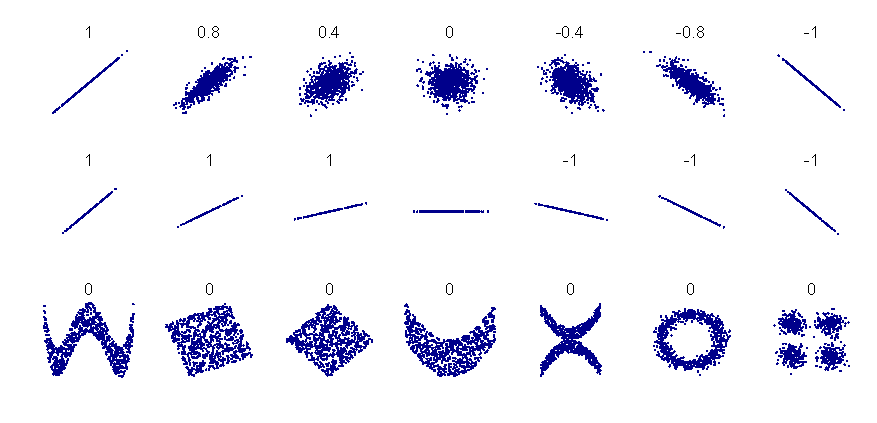
\includegraphics[width=0.8\textwidth]{figures/ch1_correlation.eps}
\caption{Several sets of $ (x,y) $  points, with the correlation coefficient of $ x $  and $ y $  for each set. Note that the correlation reflects the non-linearity and direction of a linear relationship (top row), but not the slope of that relationship (middle), nor many aspects of nonlinear relationships (bottom). (figure excerpted from \cite{www-wiki-corr})}
\label{fig:ch1_corr_ex}
\end{center}
\end{figure}


\subsection{Properties}


\subsubsection{The relation between raw moment and central moment}
The central moments $ \mu_n $  can be expressed as terms of the raw moments $ \mu_n' $ (i.e. those taken about zero) using the binomial transform \cite{papoulis2002probability}. 

\begin{thm}
The $ n $-th population central moment $ \mu_n $ can be expressed as 
\[ \mu_n = \sum_{k=0}^n \tbinom nk (-1)^{n-k} \mu_k' \mu_1'^{n-k}, \]
where $ \mu_k' $ is the $ k $-th raw moment. 
\end{thm}

\subsubsection{Moment-generating function}
Population moments, if exist, can also be obtained with \textit{moment-generating functions}. 

\begin{defn}
The moment-generating function for a random variable $ X $ is defined as 
\[ M_X(t) = \E[e^{tX}],\quad t \in \mathbb{R}, \]
whenever the expectation exists.
\end{defn}

The moments inside the function can be seen via the Taylor expansion as 
\begin{align*}
M_X(t) = \E[e^{tX}] &= \E \left [ 1+tX+\frac{(tX)^2}{2!} + \frac{(tX)^3}{3!} + \cdots \right ] \\
&= 1+ t\mu_1' + \frac{t^2}{2!} \mu_2' + \frac{t^3}{3!} \mu_3' + \cdots .
\end{align*}
By taking the $ n $-th order derivative and setting $ t=0 $, the term with $ \mu_n' $  with be left out while other terms vanish. Therefore, we have
\begin{equation}
\mu_n' = \E[X^n] = \frac{d^n M_X(0)}{dt^n}.
\end{equation}






% !TEX TS-program = latex
% !TEX root = Thesis_Guo2013.tex

\chapter{Diverging Moments and Their Asymptotics}
In the previous chapter, we have revisited some of the basic concepts in probability and outlined the definition for sample and population moments, along with some of their mathematical properties. In this chapter, we will first clarify the relation between the sample and population moments under convergence and use it as an intuition towards the central topic in this thesis, i.e. the analysis of diverging moments. Then, in the scenario of diverging population moments, we will analyze the behavior of sample moments with the growth of population size. Next, the equiprobable-slice method will be proposed, which is to serve as the key to the asymptotic analysis of diverging moments. When moments converge, the method will be shown to be consistent with the true value of moments; when moments diverge, we will see how to the method to reproduce the asymptotics of divergence.

\section{The relation between sample and population moment under convergence}
For the sake of simplicity, we restrict the moments discussed here to \textit{raw moments}, i.e. moments taken about $ c=0 $. The conclusions can also be applied to moments taken about any other value. Let us consider a random variable $ X $ and assume that its $ k $-th population raw moment $ \mu_k' $  is convergent. Supposing the population distribution is characterized by a PDF $ f(x) $, then $ \mu_k' = \int_{-\infty}^{+\infty} x^kf(x)dx $.

Now supposing we have $ N $ independent and identical distributed (i.i.d.) samples $ X_1, X_2, \cdots, X_N $, we can compute the corresponding sample raw moment as $ m_k' = \frac{1}{N} \sum_{i=1}^N X_i^k $. The distribution of each sample is obviously identical to the population distribution, therefore we have 
\begin{equation*}
\E[m_k'] = \frac{1}{N} \sum_{i=1}^N \E[X_i^k] = \frac{1}{N} \sum_{i=1}^N \int_{-\infty}^{+\infty} x_i^k f(x) dx = \mu_k',
\end{equation*}
which can be equally stated as the theorem below.

\begin{thm}
The sample moment $ m_k' $ is an unbiased estimator for the corresponding population moment $ \mu_k' $, given that $ \mu_k' $ exists (is convergent).
\end{thm}

As sample moments are computed from samples, they are random variables by themselves. Then how can one make the estimation for population moment as precise as possible? It is straightforward to imagine that a sample moment  coming from samples of a large size would be a better estimation than one from a small size. Hence, when the sample size $ N \rightarrow \infty $, can we guarantee that the sample moment equates with population moment? The answer is $ yes $ due to the \textit{Law of Large Numbers}.

\begin{thm}
(The Weak Law of Large Numbers) Let $ X_1, X_2, \cdots, X_N $ be a sequence of independent and identically distributed random variables, each having the same expectation $ \E[X_i]=\mu $ \footnote{An assumption of finite variance $\sigma(X_1)^2 = \sigma(X_2)^2 = \cdots = \sigma^2 < \infty $ is not necessary. Large or infinite variance will make the convergence slower, but the law holds anyway. This assumption is often used because it makes the proofs easier.}
, then their arithmetic mean $ \overline{X}_N = \frac{1}{N} \sum_{i=1}^{N} X_i$ converges in probability towards $ \mu $, i.e. $\lim_{N \rightarrow \infty} P(|\overline{X}_N - \mu|>\epsilon) = 0$ for any positive $ \epsilon $. 
\end{thm}

By the two theorems above, we arrive at the following lemma, which formally states the simple relation between the sample and population moment under convergence. 
\begin{lemma}
A sample moment $ m_k' $ converges in probability towards the corresponding population moment $ \mu_k' $ when the sample size $ N \rightarrow \infty $, given that $ \mu_k' $ exists (is convergent).
\end{lemma}

Fig. \ref{fig:ch2_u4converge} is an example that illustrates how this convergence is realized when the sample size grows bigger. We draw i.i.d. samples from a standard Gaussian distribution and compare the sample $ \mu_4 $ with its population counterpart $ \mu_4=3 $. The convergence is guaranteed when the sample size extends to infinity, as indicated by the trend shown here. 

\begin{figure}[htbp]
\begin{center}
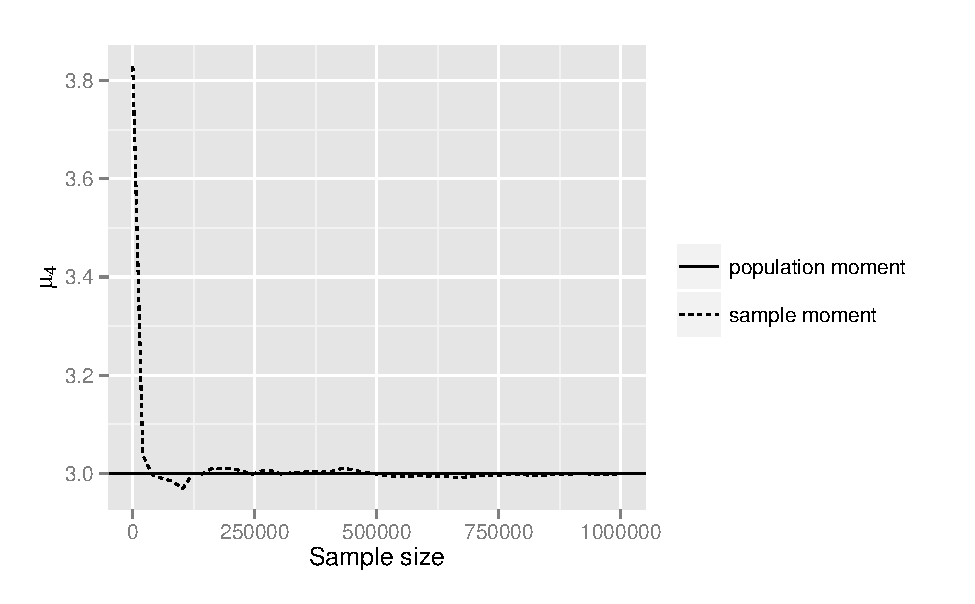
\includegraphics[width=0.9\textwidth]{figures/ch2_u4converge_gauss.eps}
\caption{Moment $ \mu_4 $ computed from i.i.d. samples of growing sample sizes drawn from a standard Gaussian distribution. It can be seen that the sample  moment converges to the population moment $ \mu_4 $ as the population size grows larger.  }
\label{fig:ch2_u4converge}
\end{center}
\end{figure}

The convergence of sample moments towards their population counterparts when they exist can also be interpreted as a consequence of the convergence of empirical distribution towards the population distribution. The empirical distribution of a sample with size $ n $ can be characterized by constructing an empirical cumulative distribution function (empirical CDF) from data.
\begin{defn}
Let $ x_1, x_2, \cdots, x_n $ be i.i.d. samples \textit{already} independently drawn from the same population CDF $ F(x) $, then the empirical CDF $ \hat{F}_n(x) $  is defined as 
\begin{equation}
\hat{F}_n(x) = \frac{\text{number of samples} \leq x}{n} = \frac{1}{n} \sum_{i=1}^n \bm{1}(x_i \leq x),
\end{equation}
where $ \bm{1}(\cdot) $ is the indicator function. 
\end{defn}

By introducing the empirical CDF, sample moments and population moments can be unified --- both of them are results of an Riemann-Stieltjes integral with the same integrand (a polynomial) but with regard to different CDFs. For example, the 4-th population raw moment is $ \int_{-\infty}^{+\infty} x^4 dF(x) $, whereas the corresponding sample moment is integrated with the empirical CDF as $ \int_{-\infty}^{+\infty} x^4 d\hat{F}_n(x) $. Meanwhile, the empirical CDf $ \hat{F}_n(x) $ is guaranteed to converge to the population CDF $ F(x) $ almost surely by the \textit{Strong Law of Large Numbers}.

\begin{thm}
(The Strong Law of Large Numbers) Let $ X_1, X_2, \cdots, X_n $ be a sequence of i.i.d. samples with the sample expectation $ \mu $, then their arithmetic mean $ \overline{X}_N = \frac{1}{N} \sum_{i=1}^N X_i$ converges almost surely to the expected value, that is $ P(\lim_{N \rightarrow \infty} \overline{X}_N = \mu) =1$.  
\end{thm}

By the Strong Law of Large Numbers, we can derive the convergence of $ \hat{F}_n(x) $ towards $ F(x) $ as below (readers interested in the proof may refer to \cite{van2000asymptotic}).
\begin{thm}
The empirical CDF $ \hat{F}_n(x) $ converges to the population CDF $ F(x) $ as $ n \rightarrow \infty$ almost surely, i.e. 
\begin{equation}
P(\lim_{n \rightarrow \infty} \hat{F}_n(x) = F(x)), \  \text{for any} \ x \in \mathbb{R}.
\end{equation}
\end{thm}

As a consequence of $ \hat{F}_n(x) \xrightarrow{a.s.} F(x) $, the convergence of sample moment towards the population counterpart is guaranteed, also in the \textit{almost surely} sense. Fig. \ref{fig:ch2_ecdf_converge} is an illustrative example that plots three empirical CDFs constructed with different sample sizes along with the population CDF. The empirical CDF with a bigger sample size conforms better to the population CDF. 

\begin{figure}[!h]
\begin{center}
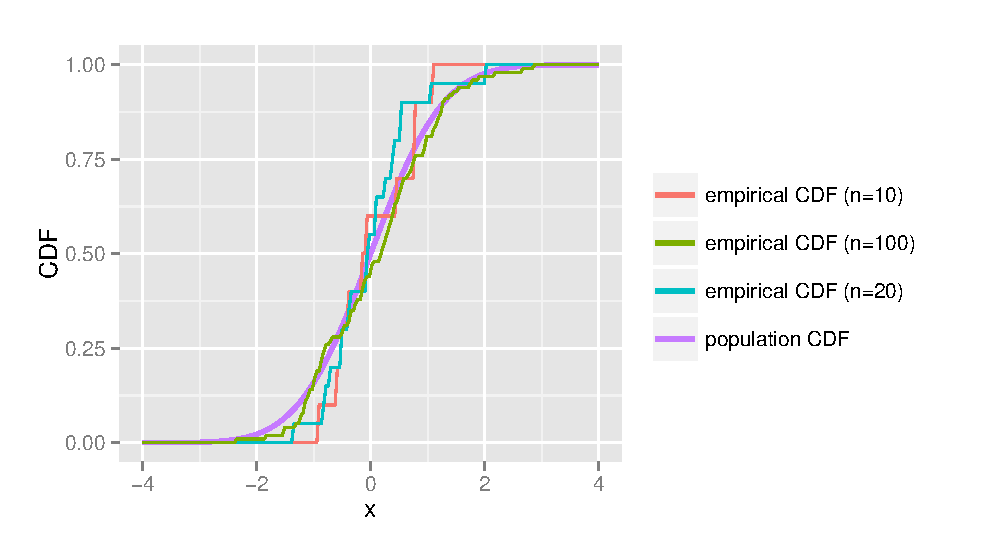
\includegraphics[width=0.9\textwidth]{figures/ch2_ecdf_converge.eps}
\caption{The CDF for the standard Gaussian distribution, accompanied with empirical CDF constructed from sample drawn from the distribution of sizes $ n=10$, $n=20$ and $n=100$. As one can observe from the trend, the gap between the population CDF and the empirical CDF diminishes.}
\label{fig:ch2_ecdf_converge}
\end{center}
\end{figure}

Hence, under convergence, sample moments obtained from a sample with large size are precise estimators for the corresponding population moments, which can be further used to estimate the parameter for the population distribution, which is called \textit{the method of moments}. 

\subsubsection{The method of moments}

Supposing the population distribution  for $ X $ is believe to be $ f(x; \theta_1, \theta_2, \cdots, \theta_p) $, where $ \theta_1, \theta_2, \cdots, \theta_p $ are the parameters to be estimated. From the distribution function, we can calculate the population moments $ \mu_1', \mu_2', \cdots, \mu_p' $, each expressed as a function of $ \theta_1, \theta_2, \cdots, \theta_p $, i.e.
\begin{equation}
\begin{split}
&\mu_1'(\theta_1, \theta_2, \cdots, \theta_p) = \int_{-\infty}^{+\infty} x f(x; \theta_1, \theta_2, \cdots, \theta_p) dx, \\
&\mu_2'(\theta_1, \theta_2, \cdots, \theta_p) = \int_{-\infty}^{+\infty} x^2 f(x; \theta_1, \theta_2, \cdots, \theta_p) dx, \\
&\vdots \\
&\mu_p'(\theta_1, \theta_2, \cdots, \theta_p) = \int_{-\infty}^{+\infty} x^p f(x; \theta_1, \theta_2, \cdots, \theta_p) dx.
\end{split}
\end{equation}
Then we collect the sample moments $ m_1', m_2', \cdots, m_p' $ from data with a large sample size. By equating every population with the corresponding sample moment, we have the equations
\begin{equation}
\begin{split}
&\mu_1'(\theta_1, \theta_2, \cdots, \theta_p) = m_1',\\
&\mu_2'(\theta_1, \theta_2, \cdots, \theta_p) = m_2', \\
&\vdots \\
&\mu_p'(\theta_1, \theta_2, \cdots, \theta_p) = m_p',
\end{split}
\end{equation}
the solution to which provide an estimation for the parameters. And this method of parameter estimation is called the method of moments.

However, the method of moments have been largely superseded by the method of \textit{maximum likelihood estimation} (MLE), which generally gives estimators with a  bigger probability of being close to the parameters to be estimated. Yet, the method of moments can yield the results more quickly and easily by solving the equation, while the MLE may take more time solving an optimization. 

\section{Diverging moments caused by heavy tails}
Previously, we have studied the asymptotic convergence (\textit{asymptotic} in the sense that the sample size $ n \rightarrow \infty $ ) relation between sample and population moments when they exist. Now it is time to move on to exploring the case when population moments diverge. We will see that the divergence of moments is caused by the heavy tails of a distribution, where the probability mass declines to zero with a pace slower than an exponential tail (e.g. the tails in Gaussian). An important member in the heavy-tailed family is the power-law distribution and we will discuss its definition, properties and empirical studies in detail. Meanwhile, it is possible for a heavy-tailed distribution has convergent lower-order moments but divergent higher-order moments. So let us first explore how the \textit{order} of a moment matters. 

% In this case, although we cannot obtain population moments, we can still calculate sample moments from data, as every data point is a finite number. By analyzing the dependence of sample moments on the sample size $ n $, we will see that sample moments \textit{grow with} $ n $. Therefore, we would ask \textit{how fast} does a sample moment grow with sample size, which can be more formally put as the \textit{asymptotic behavior} of a sample moment. Furthermore, is their anyway we can recover (or predict) the asymptotic behavior of a sample moment directly from the population distribution? 
   

\subsection{Moment order}
The theorem below states that for a distribution, if a moment of higher order exists, then every moment of lower order also exists.

\begin{thm}
For a random variable, if the $ n $-th population moment $ \mu_n' $ exists, then  for every $ 0<k \leq n $, $ \mu_k' $ also exists. 
\end{thm}
\begin{proof}
Supposing a random variable $ X $ with PDF $ f(x) $, then
\[ \mu_k' = \int_{-\infty}^{+\infty} x^k f(x) dx \leq \int_{-\infty}^{+\infty} {|x|}^k f(x) dx = \int_{|x|>1} {|x|}^k f(x) dx + \int_{|x|\leq 1} {|x|}^k f(x) dx, \]
where the first term satisfies 
\[ \int_{|x|>1}|x|^k f(x) dx \leq \int_{|x|>1} |x|^n f(x) dx = \int_1^{+\infty} x^n f(x) dx \pm \int_{-\infty}^{-1} x^n f(x) dx, \]
where both terms on RHS are convergent due to the existence of $ \mu_n' $. Meanwhile, it follows that
\[ \int_{|x| \leq 1} |x|^k f(x) dx \leq \int_{-\infty}^{+\infty} f(x) dx = 1. \] Therefore, $ \mu_k' $ is convergent.
\end{proof}

More generally, the existence of $ \mu_n' $ guarantees the convergence of $ \mu_k(c), \ 0<k \leq n $ for any $ c $. Hence, for a distribution, the convergence of moments falls into either category:
\begin{enumerate}
\item There exists a maximum order $ n_c $ for moment to be convergent. Moments with orders less than $ n_c $ are all convergent, while moments with orders higher than $ n_c $ are all divergent.
\item Moments of all orders are convergent ($ n_c=\infty $ ).
\end{enumerate}

The convergence of moment is only a problem when a distribution has a tail (the range of distribution extends to infinity on one side) or has two tails (the range extends to infinity on both sides); distributions with $ x $ bounded to a finite range always have convergent moments. By recalling how an improper integral is defined, we can see that the convergence of a population moment solely depends on the \textit{shape of its tail (or tails)}. For distributions with exponentially bounded tails, $ n_c = \infty $; for heavy-tailed distributions, we can expect $ n_c < \infty $.  

\subsection{Heavy-tailed distribution}
Supposing the CDF for a function is $ F(x) $, then a distribution (not limited to a finite range) is said to have an exponentially bounded \textit{right tail} if there exists some $ \lambda>0 $ such that 
\begin{equation}
\lim_{x \rightarrow +\infty} e^{\lambda x} (1-F(x)) < \infty,
\end{equation}
or an exponentially bounded \textit{left tail} if there exists some $ \lambda >0 $ such that 
\begin{equation}
\lim_{x \rightarrow -\infty} e^{- \lambda x} F(x) < \infty.
\end{equation}
As the definitions above imply, an exponentially bounded tail vanishes to zero as fast as an exponential function with some $ \lambda>0 $ or faster than that. Either left or right, exponentially bounded tails guarantee the existence of moments of all positive orders, i.e. $ n_c = \infty $, which is an immediate result from that $ \lim_{x \rightarrow \infty} e^{-x} x^n = 0 $ holds for any $ n $. 

However, if a tail vanishes to zero slower than $ any $ exponential function with $ \lambda>0 $, we call it a heavy-tail and it causes moments with order higher than some $ n_c $ diverge. For the sake of simplicity, we restrict tails discussed here to be \textit{right tails}, which can be extended to left tails in a similar fashion. 

\begin{defn}
The distribution of a random variable $ X $ with its CDF $ F(x) $ is said to have a heavy tail if 
\begin{equation}
\lim_{x \rightarrow +\infty} e^{\lambda x} (1-F(x)) = \infty \quad \text{for all} \ \lambda > 0.
\end{equation}
\end{defn}
This definition is equivalent to the statement that the moment generating function $ M(t) $ is infinite for any $ t>0 $ \cite{rolski2009stochastic}. 

Some common distributions with heavy-tails are listed as below.\\
Those that are one-tailed include
\begin{itemize}
\item the power-law distribution (also referred to as \textit{Pareto distribution}),
\item the log-normal distribution,
\item the Levy distribution.
\end{itemize}
Those that are double-tailed include
\begin{itemize}
\item the Cauchy distribution,
\item the t-distribution.
\end{itemize}

As a typical example of heavy-tail with both abundant empirical evidence and theoretical studies, we now briefly outline the definition and properties of \textit{power-law distributions}, which are also referred to as \textit{Pareto distributions}. 

\subsubsection{Power-law distribution}
For the sake of simplicity, we assume the random variable here to be continuous. For a random variable $ X $ obeying power-law distribution, its PDF is in the form of
\begin{equation}
f(x) = \frac{\alpha -1}{x_{\min}} (\frac{x}{x_{\min}})^{-\alpha}, 
\end{equation}
where $ x $ is defined on the range $ [x_{\min}, +\infty) $ and $ x_{\min}>0 $ is a cut-off on the minimum value for $ X $. $ \alpha>1  $ is called the \textit{scaling exponent}, its value being bigger than $ 1 $ is required for power-law to be normalizable.

The name \textit{scale exponent} is due to a property of power-law called \textit{scale invariance}. Scaling the variable $ X $ by a positive constant $ c $ only causes a proportionate scaling of the PDF itself, that is 
\begin{equation}
f(cx) = c^{-\alpha} f(x),
\end{equation}
where $ \alpha $ characterizes the power of the homogeneous function. Therefore, two power-laws with the same scaling exponent are equivalent up to a constant factor, with one being a \textit{scaled} version of the other. To simplify the expression for the PDF, one can scale $ X $ by dividing it by $ x_{min} $. Then the resulting random variable $ X' = X/x_{min} $ has the PDF with the same $ \alpha $, i.e.
\begin{equation}
f_{X'}(x) = (\alpha-1) x^{-\alpha}.
\end{equation}

\begin{figure}[!h]
\begin{center}
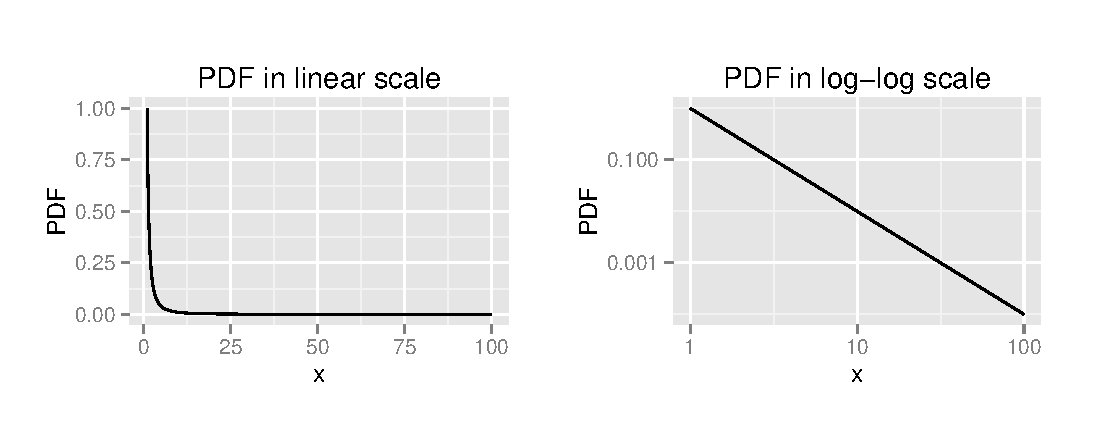
\includegraphics[width=0.9\textwidth]{figures/ch2_powerlaw_pdf.eps}
\caption{The PDF for a power-law with $ x_{\min}=1 $ and $ \alpha=2 $. The figure on the left in plotted in linear-linear scale and the figure on the right is plotted in log-log scale.}
\label{fig:ch2_powerlaw_pdf}
\end{center}
\end{figure}

Fig. \ref{fig:ch2_powerlaw_pdf} shows the PDF for a power-law distribution in two drawing scales. As the tail for power-law is heavier than a exponential one, the length of the power-law tail can be very long (the maximum of $ x $ in data can be very big) compared to the length of the head, where most of the ``probability mass'' is concentrated. Hence, a power-law is often preferred to be drawn in a log-log scale. By taking logarithm on both sides of the PDF, we can see that the logarithm of the PDF is related to the logarithm of the variable in a linear relation, with the slope being just $ -\alpha $, i.e.
\begin{equation}
\log f(x) = -\alpha	\log (x) + \log[(\alpha-1) x_{\min}^{\alpha-1}].
\end{equation}
Meanwhile, to see if a variable follows a power-law from data, it is often handy to plot the probability versus the value in log-log scale and see if is basically a straight line. However, without a following rigorous treatment for parameter estimation and statistical test, a naive graphical method for identifying power-law and estimating the exponent can be misleading \cite{Clauset2009}. 

To observe the heavy tail for power-law more straightforwardly, we can integrate the PDF to arrive at the CDF as 
\begin{equation}
F(x) = 1 - (\frac{x}{x_{\min}})^{1-\alpha}.
\end{equation}
It follows that for any $ \lambda>0 $ we have 
\[ \lim_{x \rightarrow +\infty} e^{\lambda x} (1-F(x)) = \lim_{x \rightarrow +\infty} \frac{e^{\lambda x}}{(x/x_{\min})^{\alpha-1}} =0,\]
thus proving that the tail is indeed heavier than an exponential one. 
The \textit{tail distribution} for power-law is given by
\begin{equation}
P(X>x) = 1-F(x) = (x/x_{\min})^{1-\alpha}, 
\end{equation}
which is also a relation expressed by multiplicative power. This form of characterization is often seen when the power-law is called the \textit{Pareto distribution} and the constant $ \beta=\alpha-1 > 0 $ is called the \textit{Pareto index}.

The scaling exponent $ \alpha $ (or the Pareto index $ \beta=\alpha-1 $) characterizes the \textit{heterogeneity} of a power-law distribution. As drawn in Fig. \ref{fig:ch2_alpha}, when $ \alpha \rightarrow \infty $, the distribution approaches to a Dirac delta function, with all probability mass places on a single point, which corresponds to maximal heterogeneity; when $ \alpha \rightarrow 1 $, loosely speaking, the distribution approaches a ``uniform'', where the probability mass is equally places from $ x_{\min} $ to $ \infty $, which corresponds to maximal homogeneity. 

\begin{figure}[!h]
\begin{center}
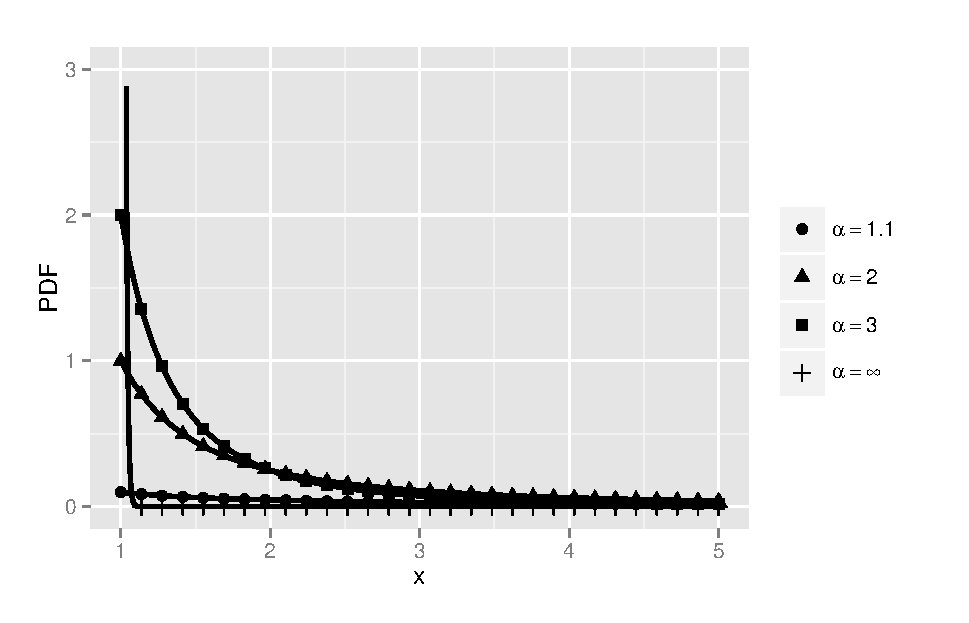
\includegraphics[width=0.9\textwidth]{figures/ch2_alpha.eps}
\caption{PDFs of power-law distributions with $ x_{\min}=1 $ and different values of $ \alpha $. It can be seen that the distribution approaches an uniform distribution when $ \alpha \rightarrow 1 $ (more homogenous), while it approaches a Dirac delta function centered at a single point when $ \alpha \rightarrow \infty $ (more heterogeneous).   }
\label{fig:ch2_alpha}
\end{center}
\end{figure}

Power-law distributions (i.e. Pareto distributions) has been empirically found in an extraordinarily diverse phenomena. Power-law is often connected with the intuition that the data is not centered around a ``typical value'', which is often referred to as \textit{heterogeneity}  For example, the distribution of population of cities and towns is found to follow a power-law: the largest city in US is New York City with more than 8 million residents but the smallest one in US is a small town with about 50 residents only \cite{newman2005power}. The distribution for the population of cities from the US Census in 2000 is drawn by Fig. \ref{fig:ch2_population}, where the straight line in log-log scale matches the form of power-law. Aside from city population, the distributions for the sizes of earthquakes \cite{gutenberg1942earthquake}, solar flares \cite{lu1991avalanches}, the frequency of words in any human language \cite{zipf1949human}, the number of citations received by papers \cite{de1965networks}, the degrees of web pages on the Internet \cite{barabasi1999emergence,faloutsos1999power}, the sales of books and recordings \cite{cox1995concentration}, people's annual incomes \cite{pareto1964cours} have also been found to follow the power-law. 

\begin{figure}[!h]
\begin{center}
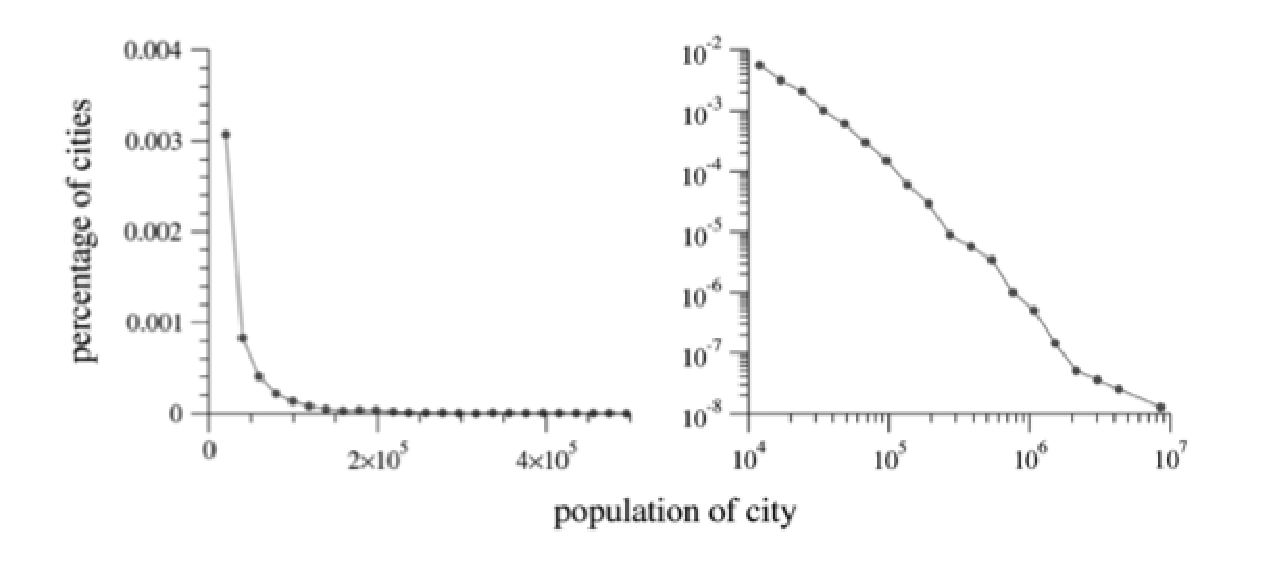
\includegraphics[width=0.9\textwidth]{figures/ch2_population.eps}
\caption{Left: histogram of the populations of all US cities with population of 10000 or more. Right: another histogram of the same data, but plotted on logarithmic scales. The approximate straight-line form of the histogram in the right panel implies that the distribution follows a power law. Data is collected from the 2000 US Census. (figure excerpted from \cite{newman2005power}))}
\label{fig:ch2_population}
\end{center}
\end{figure}

We now take a look at the maximum order $ n_c $  allowed in a power-law for a moment to converge. The $ k $-th raw moment is given by 
\begin{align*}
\mu_{k}' &= \int_{x_{\min}}^{+\infty} \frac{\alpha-1}{x_{\min}} (\frac{x}{x_{\min}})^{-\alpha} x^k dx \\
&= (\alpha-1) x_{\min}^{\alpha-1} \int_{x_{\min}}^{+\infty} x^{k-\alpha} dx = (\alpha-1) x_{\min}^{\alpha-1} \frac{x^{k-(\alpha-1)}}{k-(\alpha-1)} \Bigg|_{x_{\min}}^{+\infty},
\end{align*}
which requires $ \lim_{x \rightarrow +\infty} x^{k-(\alpha-1)} $ to converge. Therefore, we have 
\begin{equation}
k < n_c = \alpha -1
\end{equation}
for a power-law with scaling exponent $ \alpha >1 $. Notably, when $ 2 < \alpha \leq 3 $, the power-law has finite mean but diverging variance; when $ 1 < \alpha \leq 2 $, even the mean diverges.  

\section{Equiprobable partition method}
In this section, we will develop the \textit{equiprobable partition method} (EPM) as a theoretical tool for analyzing the asymptotics of diverging moments. The equiprobable partition method partitions the area under the PDF into slices with equal sizes (i.e. equal probabilities) and use these slices to represent or approximate the samples. We will see that when the moment is convergent, the sample moments given by EPM is consistent with its expectation, i.e. the corresponding population moment (that is to say, EPM is precise in the convergent case); and when the moment is divergent, we can use EPM to reproduce the asymptotic behaviors of the sample moments as the sample size grows. 

Before we go in depth to the method, we shall first explain what happens to sample moments when the corresponding population moments diverge and what we mean by using the word \textit{asymptotics} for sample moments. 

As an illustrative example, we draw ``bags'' of samples from a power-law distribution with $ x_{\min}=1 $ and $ \alpha=2.5 $, where the sample size $ n $ for the ``bag'' is growing. 
\begin{figure}[!h]
\begin{center}
\includegraphics[width=0.7\textwidth]{figures/ch2_moment_grow.eps}
\caption{Sample raw moments $ m_1', m_2', m_3' $ and $ m_4' $  computed from samples drawn from a power-law distributions with $ x_{\min}=1 $ and $ \alpha=2.5 $, plotted against the sample size $ n $ in the log-log scale .  }
\label{fig:ch2_moment_grow}
\end{center}
\end{figure}
Fig. \ref{fig:ch2_moment_grow} draws the sample raw moments $ m_1', m_2', m_3' $ and $ m_4' $ versus size of samples for computing them. Due to $ \alpha=2.5 $, the maximum order for moment to converge is $ n_c = \alpha-1=1.5 $. Therefore, as shown in the figure, only $ m_1' $ converges to its expectation $ \frac{\alpha -1}{\alpha -2}=3 $. Other moments $ m_1' $, $ m_2' $ and $ m_3' $ clearly \textit{grows with the sample size} (although the growth may look unsteady with fluctuations, the general increasing trend is obvious by referring to the exponentially spaced numbers on the y-axis). In other words, instead of converging to a fixed value, these sample moments continue to grow as more data is accumulated. The growth of a divergent sample moment relying on the sample size $ n $ when $ n \rightarrow \infty $ is what we call the \textit{asymptotic behavior} of the sample moment, or its \textit{asymptotics}. With the aid of \textit{equiprobable partition method}, we can approximate a diverging moment in the form of $ n^{\gamma} g(n) $, where $ n^{\gamma} $ characterizes the \textit{leading order} of divergence (thus answering: \textit{how fast is the divergence?} ) and $ g(n) < \infty \ (n \rightarrow \infty ) $ is a function of $ n $ that characterizes the sample moment's ``convergence'' by cutting off the divergence (thus answering: \textit{what is left in the moment other than the leading order?}).

\subsection{Equiprobable partitions}
Similar to the \textit{partition} defined in Riemann integrals (or Riemann-Stieltjes integrals), a \textit{equiprobable partition} is a list of points that cut the range for $ x $ into consecutive intervals. But, as its name suggests, the equiprobable partition is special in that it cuts the $ x $-axis in the way that the area of the PDF above every interval is \textit{the same}, so that a random sample falls into every interval with \textit{equal probability}. We will discuss why we choose such a partition scheme later.

Let us denote a partition that produces $ n $ intervals with $ \mathcal{P}_n $, which is called a \textit{$ n $-separated partition}.  The partition $ \mathcal{P}_n $ for a random variable defined on the interval $ [a,b] $ is defined as below.
\begin{defn}
Let $ X $ be a continuous random variable defined on the interval $ [a, b] \in \mathbb{R} $ with the PDF $ f(x)\ (a \leq x \leq b) $, then its $ n $-separated partition $ \mathcal{P}_n (a,b) $ is defined as 
\begin{equation}
\mathcal{P}_n (a,b) = (\hat{t}_0, \hat{t}_1, \cdots, \hat{t}_n),
\end{equation}
where $ \hat{t}_0 = a $, $ \hat{t}_n=b $ and it satisfies that 
\begin{equation}
\int_{\hat{t}_i}^{\hat{t}_{i+1}} f(x) dx = \frac{1}{n} \quad (i=1,2,\cdots, n-1).
\end{equation}
\end{defn}

It directly follows from the definition that the interval points can be obtained from the CDF $ F(x) $ as
\begin{equation}
F(\hat{t}_i) = \frac{i}{n} \quad (i=0,1,\cdots,n)
\end{equation}
If we assume that the PDF $ f(x) $ is a well-defined function, then its integral $ F(x) $ should be an increasing function, of which the inverse function $ F^{-1}(x) $ must exist. The interval points can thus be uniquely determined by the inverse function of CDF, i.e.
\begin{equation}
\hat{t}_i = F^{-1} (\frac{i}{n}) \quad (i=0,1,\cdots, n).
\end{equation}
Fig. \ref{fig:ch2_partition_schematic} is a schematic illustration of a partition $ \mathcal{P}_n(a,b) $ with $ n=9 $. Clearly, the interval points are not evenly spaces. Instead, the density for interval points is high when $ f(x) $ is large and is low when $ f(x) $ is small, which is consistent with how samples are distributed in regions with different probability densities. 
\begin{figure}[htbp]
\begin{center}
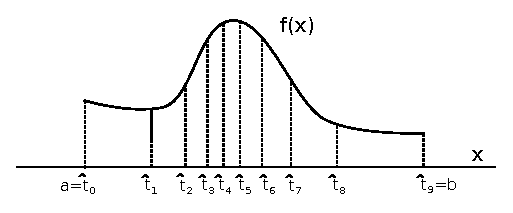
\includegraphics[width=0.9\textwidth]{figures/ch2_partition_schematic.eps}
\caption{A schematic of illustration of $ P_9(a,b) $. Instead, the density for interval points is high when f(x) is large and is low when f(x) is small, which is consistent with how samples are distributed in regions with different probability densities.}
\label{fig:ch2_partition_schematic}
\end{center}
\end{figure}

Hence, we can use the interval points in equiprobable partitions to \textit{approximate sample points}. In the Riemann integral, one point picked in each interval in the partition as the \textit{representative point} for that interval, and the partition is said to be \textit{tagged} by these representative points. How one picks the representative points does not matter as long as the Riemann sum converges when the maximum length of intervals diminishes to zero. Similarly, in our case, to every interval we assign a representative point placed in the interval. As the positioning of this point inside the interval does not matter when $ n \rightarrow \infty $, for convenience, we just pick the left end $ \hat{t}_{i} $ for the interval $ [\hat{t}_i, \hat{t}_{i+1}] $ as the \textit{representative point} .  

Now, we use $ n $ representative points $ \{ \hat{t}_0, \hat{t}_1, \cdots, \hat{t}_{n-1} \}$ derived from an $ n $-separated equiprobable partition to approximate a sample $ \{ x_1, x_2, \cdots, x_n \} $ of size $ n $. That is to say, the set of points $ \{ \hat{t}_0, \hat{t}_1, \cdots, \hat{t}_{n-1} \} $ as a whole is an approximation for the set of samples $ \{x_1, x_2, \cdots, x_n\} $ as a whole, while the ordering among the elements in each does not matter. 

Meanwhile, because we know that $ \hat{t}_0 \leq \hat{t}_1 \leq \cdots \leq \hat{t}_{n-1} $, we first sort the samples and then use $ \hat{t}_{i} $ as an approximation for the $ (i+1) $-th smallest sample. In other words, the determinant points $ (\hat{t}_0, \hat{t}_1, \cdots, \hat{t}_{n-1}) $ can be used to estimate the \textit{order statistics} for a distribution, where both the ordering among $ \{\hat{t}_i\} $  and the ordering among samples after sorting shall be taken into account.

For now, we focus on the first case where ordering does not matter. By using $\{ \hat{t}_0, \hat{t}_1, \cdots, \hat{t}_{n-1} \}$ to approximate the samples $ \{ x_1, x_2, \cdots, x_n \} $, we seek to construct estimators for sample moments. 

\subsection{EPM estimators for sample moments}
Every sample moment taken at point $ c $ is a polynomial function of sample points, i.e.
\begin{equation}
m_{k}(c) = \frac{1}{n} \sum_{i=1}^{n} (x_i-c)^k.
\end{equation}
The EPM (equiprobable partition method) estimator for the sample moment is constructed by simply \textit{replacing the samples $ \{x_1, x_2, \cdots, x_n\} $ with the representative points $ \{ \hat{t}_0, \hat{t}_1, \cdots, \hat{t}_{n-1} \} $}.  

\begin{defn}
Given a random variable $ X $ and a sample of size $ n $ independently drawn from its distribution, the EPM (equiprobable partition method) estimator for the $ k $-th sample moment $ m_k(c) $ is defined to be
\begin{equation}
\hat{m}_k(n;c) = \frac{1}{n} \sum_{i=1}^{n} (\hat{t}_{i-1}-c)^k,
\end{equation}
which is a function of $ n $. The interval points $ \{ \hat{t}_0, \hat{t}_1, \cdots, \hat{t}_{n} \} $ are given by the $ n $-separated equiprobable partition $ \mathcal{P}_n $ for $ X $. 
\end{defn}

We now show that when $ X $ is a random variable defined on a finite interval and its PDF is bounded. Then the EPM moment estimator is \textit{unbiased} when $ n \rightarrow \infty $, that is it coincides with population moment. We will show that, in fact, an EPM moment estimator is in fact the same as the Riemann-Stieltjes integral for the corresponding population moment when $ n $ extends to infinity.

\begin{thm}
Let $ X $ be a random variable defined on the interval $ [a, b] $ with its PDF $ f(x) \  (a \leq x \leq b) $. Supposing $ f(x) $ is bounded, i.e. there exists some $ M $ that it holds that $\forall x \in [a, b]$, $f(x) < M$, we have 
\begin{equation}
\lim_{n \rightarrow \infty} \hat{m}_{k}'(n) = \mu_k',
\end{equation}
where $ \hat{m}_{k}'(n) = \frac{1}{n} \sum_{i=1}^n (\hat{t}_{i-1})^k $ is the EPM estimator for $ k $-th raw moment, $ \mu_k' $ is the $ k $-th population moment. \label{thm:epm_consistent}
\end{thm} 

\begin{proof}
From the definition of $ \mathcal{P}_n(a,b) $, we have
\begin{align*}
\frac{1}{n} &= F(\hat{t}_i) - F(\hat{t}_{i-1}) \quad (i=1,2,\cdots,n) \\
&= f(\hat{t}_{i-1})(\hat{t}_i - \hat{t}_{i-1}) + o(\hat{t}_{i}-\hat{t}_{i-1}).
\end{align*}
For an $ \epsilon>0 $ that is small enough, if $ \hat{t}_i - \hat{t}_{i-1} < \epsilon $, then we have $ o(\hat{t}_{i}-\hat{t}_{i-1}) < \delta (\hat{t}_i - \hat{t}_{i-1}) $ for some $ \delta>0 $. Meanwhile, due to the bound $ f(x)<M $, we have
\[ \frac{1}{n} < (M+\delta)(\hat{t}_{i}-\hat{t}_{i-1}). \]
Therefore, for any small $ \epsilon>0 $, when $ n > \frac{1}{(M+\delta)\epsilon} $, we shall have $ (\hat{t}_i - \hat{t}_{i-1})<\epsilon $. That is, 
\[ \lim_{n \rightarrow \infty} \max_{1 \leq i \leq n} (\hat{t}_i - \hat{t}_{i-1}) = 0, \]
showing that the \textit{mesh} for the partition vanishes to zero when $ n \rightarrow \infty $.  
Meanwhile, the EPM estimator can be rewritten as
\begin{align*}
\lim_{n \rightarrow \infty} \hat{m}_k'(n) &= \lim_{n \rightarrow \infty} \frac{1}{n} \sum_{i=1}^n (\hat{t}_{i-1})^k \\
&= \lim_{n \rightarrow \infty} \sum_{i=1}^n (\hat{t}_{i-1})^k [F(\hat{t}_i) - F(\hat{t}_{i-1})].
\end{align*}
Hence, by the definition of Riemann-Stieltjes integral, we have 
\[ \lim_{n \rightarrow \infty} \hat{m}_{k}'(n) = \int_{a}^b x^k dF(x) = \mu_k'. \]
\end{proof}

By expanding a moment taken about $ c $, we arrive at the following conclusion immediately. 
\begin{lemma}
For a random variable $ X $ with bounded PDF $ f(x) < M \ (a \leq x \leq b) $, we have 
\begin{equation}
\lim_{n \rightarrow \infty}{\hat{m}_k (n)} = \mu_k,
\end{equation}
\begin{equation}
\lim_{n \rightarrow \infty}{\hat{m}_k (n;c)} = \mu_k(c).
\end{equation}
\end{lemma}
That is to say, the EPM estimators for sample central moments or moments taken about any point coincide with population moment, if $ X $ is a random variable with finite range and bounded PDF. To arrive at these conclusions, we have assumed that the PDF is bounded, which applies to most well-defined distributions and only rules out those with \textit{generalized functions} (e.g. PDFs containing Dirac's delta).

\subsection{Asymptotics for diverging moments}
Having proven that EPM estimators are \textit{precise} when moments converge, we now extend the usage of EPM estimators to deriving the asymptotics of diverging sample moments. For convenience, in this section we assume that $ X $ is a random variable \textit{with a heavy tail on the right side}, while right-tailed or double-tailed distributions can be analyzed in a similar fashion. Let $ f(x) \ (a \leq x < +\infty) $ be the PDF for $ X $ and $ f(x)$ is bounded by some $ M $. The equiprobable partition for $ X $ is defined by changing $ \mathcal{P}_n(a,b) $ to $ \mathcal{P}_n(a, +\infty) $, that is
\begin{equation}
\mathcal{P}_n(a, +\infty) = (\hat{t}_0, \hat{t}_1, \cdots, \hat{t}_{n-1}, \hat{t}_n),
\end{equation}
where $ \hat{t}_0=a $ and $ \hat{t}_{n}=+\infty $. The representative points $ \{\hat{t}_0, \hat{t}_1, \cdots, \hat{t}_{n-1}\} $ are given by 
\begin{equation}
F(\hat{t}_i) = \frac{i}{n} \quad (i=0,1,\cdots,n-1),
\end{equation}
where it shall be noted that the probability mass from the maximum representative to infinity is also $ 1/n $. That is to say, the EPM imposes an upper cut-off on approximated samples and the probability of drawing a random sample beyond the cut-off is $ 1/n $, which vanishes to zero when $ n \rightarrow \infty $. 
  
The $ k $-th sample moment $ m_k(c) $ computed from a sample of size $ n $ is approximated by the EPM estimator $ \hat{m}_k(n;c) $, which is constructed by substituting the sample points with representative points from the $ n $-separated equiprobable partition, i.e.
\begin{equation}
\hat{m}_k (n;c) = \frac{1}{n} \sum_{i=1}^n (\hat{t}_{i-1}-c)^k.
\end{equation}

Then, we rewrite $ \hat{m}_k(n) $ ($ c $ is left out for simplicity) into the form of 
\begin{equation}
\hat{m}_k(n) = n^{\gamma} g(n),
\end{equation}
where $ n^\gamma $ is the \textit{leading order} that characterizes the speed of convergence. And $ g(n) $ is a function that satisfies 
\begin{equation}
0 < \lim_{n \rightarrow \infty} |g(n)| < \infty,
\end{equation}
which is the ``convergent term'' for sample moments formed by deducting the effect of divergence from the sample moment.

To showcase the analytical procedure above, we use this machinery to find the asymptotics for the first several diverging moments of the power-law distributions with $ \alpha < 3 $ and compare them to numerical results. 

Here we assume the lower cut-off $ x_{\min}=1 $, and the PDF is given by 
\begin{equation}
f(x) = (\alpha-1) x^{-\alpha},
\end{equation}
and the CDF is given by
\begin{equation}
F(x) = 1 - x^{1-\alpha}.
\end{equation}
We use the CDF to construct the $ n $-separated equiprobable partition $ \mathcal{P}_n(1, +\infty) $. From the relation
\begin{equation}
F(\hat{t}_i) = 1-(\hat{t}_i)^{1-\alpha} = \frac{i}{n} \quad (i=0,1,\cdots, n-1),
\end{equation}
we have the representative point as 
\begin{equation}
\hat{t}_i = (1-\frac{i}{n})^{-c}, 
\end{equation}
where we adopt a shorthand $ c = \frac{1}{\alpha-1} > \frac{1}{2}$. When $ \alpha \leq 3$, the maximum order for convergent moment is $ n_c=\alpha-1 < 2 $, here we present the asymptotics for diverging sample raw moments $ m_k' $ with $ k \geq 2 $.

The EPM estimator for $ m_k' $ is 
\[ \hat{m}_k'(n) = \frac{1}{n} \sum_{i=0}^{n-1} (\hat{t}_i)^k = \frac{1}{n} \sum_{i=0}^{n-1} (1-\frac{i}{n})^{-ck},\]
which can be rewritten as the product of a leading order term and a ``convergent'' term, i.e.
\begin{equation}
\hat{m}_k'(n) = \frac{1}{n} \sum_{i=0}^{n-1} n^{ck} (n-i)^{-ck} = n^{ck-1} \sum_{i=1}^n \frac{1}{i^{ck}}.
\end{equation}
Therefore, the leading order for the $ k $-th diverging raw moment is $ n^{ck-1} \ (ck>1)$, and a higher order $ k $ means a faster divergence with $ n $.  The ``convergent'' term is 
\begin{equation}
g(n) = \sum_{i=1}^n \frac{1}{i^{ck}} \quad (ck>1),
\end{equation}
and its limit is the famous \textit{Riemann zeta function}
\begin{equation}
\lim_{n \rightarrow \infty} g(n) = \zeta(ck).
\end{equation}
Therefore in limit of $ n \rightarrow \infty $, the EPM asymptotics for sample moments are given by
\begin{equation}
\hat{m}_{k}'(n) \approx n^{ck-1} \zeta(ck).
\end{equation}

\begin{figure}[!h]
\begin{center}
\includegraphics[width=0.8\textwidth]{figures/ch2_powerlaw_asymptotics.eps}
\caption{The comparison between numerical sample moments $ \hat{m}_3 $, $ \hat{m}_4 $ $ \hat{m}_5 $ (cross) and their EPM asymptotics (line). The divergence can be effectively characterized by the asymptotics. Sample moments fluctuate around the theoretical line due to randomness.}
\label{fig:ch2_powerlaw_asymptotics}
\end{center}
\end{figure}

In Fig. \ref{fig:ch2_powerlaw_asymptotics}, we compare the sample moments computed from numerical experiments with their asymptotics given by EPM for $ k=2,3,4 $. That the diverging sample moments fluctuate around their asymptotics shows that the equiprobable partition method is valid in two aspects: the leading order is correct, so that the slope matches the speed of divergence with different orders; the remaining ``convergent'' term is correct, so that the intercept match the positioning of points. 

\subsection{EPM estimators for order statistics}
As mentioned earlier, the ordering among representative points given by EPM can also be utilized to construct estimators for order statistics, i.e. the sorted samples. 

\begin{defn}
Given $ X $ as a random variable and supposing $ X_1, X_2, \cdots, X_n $ are $ n $ i.i.d. samples drawn from the distribution, then the \textit{order statistics}   ${X_{(1)}, X_{(2)}, \cdots, X_{(n)}}$ for the samples are defined by sorting the samples in the increasing order. That is $ X_{(1)}, X_{(2)}, \cdots, X_{(n)} $ is a permutation of the samples that satisfies 
\begin{equation}
X_{(1)} \leq X_{(2)} \leq \cdots \leq X_{(n)}.
\end{equation}
\end{defn}

The representative points given by an $ n $-seperated equiprobable partition naturally satisfies 
\begin{equation}
t_0 < t_1 < \cdots < t_{n-1}.
\end{equation}
Therefore, we can use the $ i $-th smallest EPM representative point to estimate the $ i $-th smallest sample, i.e.
\begin{equation}
\hat{X}_{(i)} = t_{i-1} \quad (i=1, 2, \cdots, n).
\end{equation}

For most cases in asymptotic analysis for sample moments, it is \textit{unnecessary} to use the estimators for order statistics, as sample moments are defined to be \textit{permutational invariant}. For example, the variance is the same for samples $ X_1, X_2, X_3 $ and $ X_3, X_2, X_1 $, where the ordering among samples does not matter.

Yet, the EPM estimators for order statistics is useful when addressing the statistics where the ordering among elements is concerned, e.g. those in \textit{time series}. 
In the following Chapter, we will see a scenario that applies EPM estimators to obtaining the bounds of a statistic with regard to all permutations of the time series.

\subsection{Why equiprobable}
We have introduced the equiprobable partition method and used it as an estimation for samples and order statistics. The reader may be curious about the reason behind the principle of cutting the probability mass into slices of \textit{equal probabilities}, which plays a central role in the magic of EPM. Now, instead of a rigorous argument towards its mathematical necessity, we just briefly outline the intuitive \textit{rationale} behind this principle. 

\begin{enumerate}
\item A equiprobable partition ensures that the \textit{mesh} of the partition vanishes to zero as the number of partitions increases. 

This has been proven by Theorem \ref{thm:epm_consistent} and is important to guarantee that the estimator is unbiased when the moment converges. Of course, it is possible to propose other schemes of partitioning with the same mesh-vanishing property. 

\item The equiprobable partition reaches maximum entropy. 

Let us view a partition as a way to \textit{discretize} a continuous distribution. Then, for a $ n $-separated partition, there are $ n $ outcomes with one outcome corresponding to one interval. Let $ p_i \ (i=1,2, \cdots, n)$ be the probability of a random sample falls into the $ i $-th interval, then the entropy for this discrete distribution would be 
\begin{equation}
H = -\sum_{i=1}^{n} p_i \log(p_i).
\end{equation}
And the configuration $ p_1 = p_2 = \cdots = p_n = \frac{1}{n} $, as used in EPM, is the only one that maximizes the entropy. The principle of maximum entropy has been applied in statistics, information theory and statistical mechanics and reader may refer to the discussions in \cite{jaynes1957information,jaynes1957information2,jaynes1988relation} by Jaynes.

\item It is easy to determine interval ends in the equiprobable partition. 

For most well-defined distributions, the interval ends and therefore the representative points can be easily and uniquely determined with $ F^{-1}(x) $. This is important in practical applications. 

\end{enumerate}







% !TEX TS-program = latex
% !TEX root = Thesis_Guo2013.tex

\chapter{Memory Constraints for Power-law Series}
In this Chapter, we will present an application of EPM (\textit{equiprobable partition method}) to time series analysis. With a permutational technique, we will explore the bounds for the 1st-order autocorrelation for series with different (marginal) distributions, including Gaussian, uniform and power-law. 

The 1st-order autocorrelation is a moment defined for multiple variables for characterizing the interdependence among them. Specifically, it can be used to measure the temporal memory effect for time series and it is therefore also referred to as \textit{memory} by some physicists. We found that, very interestingly, for series that follow Gaussian and uniform distributions, the bounds for memory are just the bounds allowed by its definition (natural bounds). However, interestingly, the memory for power-law series is constrained to a much narrower region that relies on the scaling exponent. With EPM, we obtained these bounds when the sample moments involved are divergent, a case that cannot be readily tackled with traditional probabilistic methods. 

\section{Memory for time series}

From a statistical point of view, a time series $ \{t_1, t_2, \cdots, t_n\} $ is a ordered sequence of random variables. Ideally, the distribution for a time series of length $ n $ can be fully characterizes by the joint distribution $ f(t_1, t_2, \cdots, t_n) $. However, for a long series, the space for this distribution is very huge that it can neither be effectively determined or compactly represented. Therefore, we split the characterization for the distribution into two aspects --- the marginal and the interdependence. 

The marginal distribution refers to how one element is distributed regardless of other elements in the series, denoted by $ f(t_1) $, $f(t_2) $, $ \cdots $, $ f(t_n) $. Practically, it is often assumed that the marginal is \textit{stable}, i.e. the marginal distribution for every element is the same and does not change with time. Hence, for example, we can plot all the elements in the series in a histogram and by its distinguished bell curve we learn the marginal is Gaussian. When we speak of Gaussian series or power-law series, we are referring to the marginal distribution.

Aside from the marginal distribution, the elements in the series are intercorrelated by themselves. That is to say, a time series is more than a collection of samples independently drawn from the same marginal. Instead, their temporal ordering affects what values the elements may take. For example, a rising or falling trend is often observed for time series in financial markets. 
And memory (1st-order autocorrelation) is introduced as a simplest measure to characterize the interdependence among these elements \cite{Goh2008}. 

For a time series $ \{t_1, t_2, \cdots, t_{n}\} $, memory is defined as the Pearson's correlation coefficient between $ \{t_{2}, t_{3}, \cdots, t_{n} \}$ and its lag-1 counterpart $ \{t_{1}, t_{2}, \cdots, t_{n-1}\} $, i.e.
\begin{equation}
	M = \frac{1}{n-1} \sum_{i=1}^{n-1} \frac{(t_i - m_1)(t_{i+1} - m_2)}{\sigma_1 \sigma_2},
\end{equation}
where $ m_1, m_2 $  and $ \sigma_1, \sigma_2 $ refer to the mean and standard deviation of the two series. Intuitively from the definition, memory describes the temporal \textit{consistency} of a series: if a big (compared to average) element tends to follow a big element and a small one tends to follow a small one, then the series is \textit{consistent} and its memory is positive; on the contrary, if a big one tends to follow a small one and a small one tends to follow a big one, then the series is \textit{inconsistent} and its memory is negative. 

Due to Cauchy-Schwartz inequality
\begin{equation}
	\left\vert M \right\vert \leq \frac{1}{\sigma_1 \sigma_2} \sqrt{\left[ \frac{1}{n-1} \sum_{i=1}^{n-1} (t_i - m_1)^2  \right] \left[ \frac{1}{n-1} \sum_{i=1}^{n-1} (t_{i+1} - m_2)^2 \right]} = 1,
\end{equation}
the natural bounds $ -1 \leq M \leq 1 $ hold for all series. The upper extreme $ +1 $ marks the maximum consistency and the minimum $ -1 $ marks the power extreme $ -1 $ marks the minimum consistency. And $ M=0 $ suggests that the series is neither consistent or inconsistent --- the series is similar to independently samples in this regard and the short-range interdependence among elements is weak.

\section{Modeling correlated series with a specified marginal}
Clearly, when every $ t_{i} $ is independently sampled from the same marginal distribution $ f(x) $ , there is no interdependence among elements and the expectation value of $ M $ is zero. To modify the interdependence structure while preserving the marginal, we first sort the independently sampled series and then reorder the samples by a permutation $ \theta $ with regard to every element's ranking in the sorted series.
The sorted series directly give us the order statistics $ \{t_{(i)}\} $, 
where $ 0 < t_{(1)} \leq t_{(2)} \leq \cdots \leq t_{(n)} $.  
Then, by applying a permutation $ \theta $ (a one-to-one mapping from the set $ \{1, 2, \cdots, n\} $ to itself) to $ \{t_{(i)}\} $, we now have a sequence $ \{t_{(\theta_{i})}\} $ with a different interdependence structure but the same marginal marginal distribution. 

For a series samples from a specified marginal, by changing $ \theta $, i.e. the way we permute them, we can expect series produced with different values of memory $ M $. For example, if series are permuted such that big elements tend to be followed by big ones and small followed by small ones, $ M $ would be positive; on the contrary, if big elements followed by small ones and small elements followed by big ones, $ M $ would be negative. 

\subsection{Permutational extremes for memory}
Interestingly, there exist fixed $ \theta_{\max} $ and $ \theta_{\min} $ that respectively maximizes and minimizes $ M $ among all possible permutations. And we can use these two extremes to derive the bounds for memory in the sense of all permuted independent samples.

To see this, we need to find out how a permutation affects $ M $. 
As the values of the two aforementioned series are different in only one element ($ t_{1} $ in head and $ t_{n} $ in tail), we assume $ m_{1} = m_{2} = m$ and
$ \sigma_{1} = \sigma_{2} = \sigma $ when $ n $ is large, where $ m $ and $ \sigma $ are the mean and standard deviation of the whole series. Then the memory  of $ \{t_{(\theta_i)}\} $ can be rewritten as
\begin{equation}
	M = \frac{1}{\sigma^2} \big( \frac{1}{n-1} \sum_{i=1}^{n-1} t_{(\theta_i)}t_{(\theta_{i+1})} - m^2 \big), \label{eqs:MSimple}
\end{equation} 
where the reordering of the series only affects the summed products of adjacent terms $ S_{\theta} = \sum_{i=1}^{n-1} t_{(\theta_i)} t_{(\theta_{i+1})} $, while leaving $ m $ and $ \sigma $ unchanged. The desired extreme permutations for $ M $ are just those maximize/minimizes $ S_{\theta} $, denoted by $ \theta_{\max} $ and $ \theta_{\min} $. It has been shown that, for any $ n $,  there are fixed $ \theta_{\max} $ and $ \theta_{\min} $ for any real numbers $ t_{(1)} \leq t_{(2)} \leq \cdots \leq t_{(n)} $ \cite{Hallin1992} \footnote{Whereas \cite{Hallin1992} uses an objective function that sums the products in a circle, i.e. $S^{\prime}_{\theta} = \sum_{i=1}^{n-1} t_{\theta_{i}} t_{\theta_{i+1}} + t_{\theta_{1}} t_{\theta_{n}}$, the results can be reduced to our case by introducing an additional $ S_0 = 0 $ to the series, which makes zero contribution to the sum.}.

$ \theta_{\max} $ obtains the maximum memory by first arranging the odd elements of order statistics in the increasing order, followed by even elements in the decreasing order, which is
\begin{equation}
\begin{split}
&t_{(1)}, t_{(3)}, \cdots, t_{(2l-1)}, t_{(2l)}, t_{(2l-2)}, \cdots, t_{(4)}, t_{(2)} \quad (n=2l), \\
&t_{(1)}, t_{(3)}, \cdots, t_{(2l-1)}, t_{(2l+1)}, t_{(2l)}, \cdots, t_{(4)}, t_{(2)} \quad (n=2l+1). \\
\end{split} \label{eqs:maxArrange}
\end{equation} 
For simplicity, we only address the case when $ n=2l $, the sum with order statistics is expressed as 
\begin{equation}
	S_{\theta_{\max}} = \sum_{i=1}^{2l-2} t_{(i)}t_{(i+2)} + t_{(2l)}t_{(2l-1)} \quad (n=2l), \label{eqs:Smax}
\end{equation}
while the case of odd $ n $ can be handled similarly.



 
On the contrary, $ \theta_{\min} $ arranges the order statistics by alternating small and big terms, i.e.
\begin{equation}
\begin{split}
&t_{(2l)}, t_{(1)}, t_{(2l-2)}, \cdots, t_{(2l-3)}, t_{(2)}, t_{(2l-1)} \quad (n=2l), \\
&t_{(2l)}, t_{(2)}, \cdots, t_{(l)}, \cdots, t_{(1)}, t_{(2l+1)} \quad (n=2l+1).
\end{split} \label{eqs:minArrange}
\end{equation}
Again, for even $ n $, we have
\begin{equation}
	S_{\theta_{\min}} = \sum_{i=1}^{l-1} \big( t_{(i)}t_{(2l+1-i)} + t_{(i)}t_{(2l-1-i)} \big) + t_{(l)}t_{(l+1)} \quad (n=2l).
\end{equation}

We then define the upper bound and lower bound for memory as the mathematical expectation of $ M $ under $ \theta_{\max} $  and $ \theta_{\min} $ respectively. And in the limit of large length of series, the bounds 
\begin{equation}
M_{\max} = \lim_{n \rightarrow \infty}\E{[M(t_{\theta_{\max}})]}
\end{equation}
and
\begin{equation}
M_{\min} = \lim_{n \rightarrow \infty}\E{[M(t_{\theta_{\min}})]}
\end{equation}
can be derived in a closed form or effectively approximated. It can be shown that $ M_{\max}=1 $ and $ M_{\min}=-1 $ hold for Gaussian and uniform distributions, corresponding the natural range of $ M $. However, a much narrower range is found for power-law distributions, where the bounds rely on the exponent $ \alpha $. It shall be noted that the bounds discussed here are tight as they are the values of $ M $ under permutations $ \theta_{\max} $ and $ \theta_{\min} $.

\section{The bounds for memory}
\subsection{Adjusting memory by iterative rearrangement}
Before an in-depth theoretical treatment, we first explore the bounds for uniform, Gaussian and power-law samples by iteratively rearranging them towards $ \theta_{\max} $ or $ \theta_{\min} $. 

To do this, we construct an approximation of the order statistic iteratively. The process contains $ n $ steps, the same as the length of the series. In each step, the series is rearranged with one pass of bubble sort on the series produced after the last step, which means stepping through the series from the first element to the last, comparing each pair of adjacent elements and swap them if they are not in increasing order. The series obtained after $ i $ such steps is denoted as $ \{ \tilde{t}^{(i)} \} $, as an approximation to the order statistics, with $ \{ \tilde{t}^{(n)} \} $ guaranteed to be the same as the order statistics because a bubble sort always finishes in $ n $ passes.

In each step, treating $ \{ \tilde{t}^{(i)} \} $ as approximate order statistics, series with positive and negative memory are obtained by rearranging $ \{ \tilde{t}^{(i)} \} $  according to (\ref{eqs:maxArrange}) and (\ref{eqs:minArrange}) respectively.

In our experiment, series are of length $ n=10,000 $, independently drawn from uniform distribution on $ [0,1] $, standard Gaussian distribution (all samples are added by the same positive constant afterwards to ensure being positive), and power-law distribution whose probability density function is
\begin{equation}
	f(t) = \frac{\alpha-1}{t_{\min}} (\frac{t}{t_{\min}})^{-\alpha},
\end{equation}
with $ t_{\min}=1 $ and $ \alpha=3.5 $.
Results are obtained by averaging 5 independent runs and reported by Figure \ref{fig:TuningUpMem} for positive memory and Figure \ref{fig:TuningDownMem} for negative memory.

\begin{figure}[!ht]
\centering
\includegraphics[width=0.7\textwidth]{figures/TuningUp-power-uni-gauss.eps}
\caption{Memory tuned up by iteratively rearranging independently sampled series.}
\label{fig:TuningUpMem}
\end{figure}

\begin{figure}[!ht]
\centering
\includegraphics[width=0.7\textwidth]{figures/TuningDown-power-uni-gauss.eps}
\caption{Memory tuned down by iteratively rearranging independently sampled series.}
\label{fig:TuningDownMem}
\vspace{1em}
\end{figure}


As can be seen, by rearranging the series towards $ \theta_{\max} $, 
the memory goes to $ +1 $ for all three distributions. 
As is noted, the maximum memory of power-law series after the last iteration is slightly below $ +1 $, 
due to the effect of finite $ n $, which we will see later. 
However, while the memory can be tuned down to $ -1 $ by rearrangement towards $ \theta_{\min} $  for uniform and Gaussian distributed series, 
it is bounded above about $ -0.2 $ for the power-law series. 
In the following sections, we will further analyze how this non-trivial lower bound depends on the exponent $ \alpha $.
\subsection{Probablistic method for the $ \alpha>3 $ case}
To derive how the bounds rely on $ \alpha $, we first consider the case where $ \alpha > 3 $, which is necessary for the population variance $ \sigma({\alpha})^{2} $ to converge, and the corresponding sample variance $ \sigma^{2} $ appear in the denominator of $ M $. When $ \alpha>3 $, by simply equating the sample moments with the corresponding population moments, we have 
\begin{equation}
	\E[M(t_{\theta})] = \frac{1}{\sigma(\alpha)^2} (\frac{1}{n-1} \sum_{i=1}^{n-1} \E[t_{\theta_i}t_{\theta_{i+1}}] -m(\alpha)^2 ), \label{eqs:Mprob}
\end{equation} 
where
\begin{equation}
	m(\alpha) = \int_{1}^{+\infty} xf(x) dx = \frac{\alpha-1}{\alpha-2},
\end{equation}
\begin{equation}
	\sigma(\alpha)^2 = \int_{1}^{+\infty} x^{2}f(x) dx - m(\alpha)^{2} = \frac{\alpha-1}{\alpha-3} - m(\alpha)^2.
\end{equation}
Here, $ f(x) = (\alpha-1)x^{-\alpha} $ is the PDF for power-law, and without loss of generality, we assume $ x_{\min}=1 $ because $ M $ would remain the same if every $ t_{i} $ is divided by the same constant.

The upper bound directly relates to $ \lim_{n \rightarrow \infty} \frac{1}{n-1} E[S_{\theta_{\max}}] $, 
where the expected value of $ S_{\theta_{\max}} $ is composed of the expected value of products of adjacent items according to equation (\ref{eqs:Smax}), i.e.
\begin{equation}
	\frac{1}{n-1}\E[S_{\theta_{\max}}] = \frac{1}{2l-1}\sum_{i=1}^{2l-2} \E[t_{(i)} t_{(i+2)}] + \frac{1}{2l-1} \E[t_{(2l)} t_{(2l-1)}], \label{eqs:s-maxmem}
\end{equation}
assuming $ n=2l $. The case when $ n=2l+1 $ can be worked out in a similar fashion to arrive at the same results.

The expected value of each term can be obtained by using the joint distribution of order statistics. 
The probability density function for the joint distribution of two order statistics $ t_{(j)}, t_{(k)}\  (j <k)$ is given by \cite{David2003}
\begin{equation}
	f_{t_{(j)}, t_{(k)}} (x,y) = n! \frac{[F(x)]^{j-1}}{(j-1)!} \frac{[F(y) - F(x)]^{k-1-j}}{(k-1-j)!} \frac{[1-F(y)]^{n-k}}{(n-k)!} f(x) f(y) \quad  (x \leq y),
\end{equation}
where $ F(x) $ is the cumulative distribution function for power-law, i.e.
\begin{equation}
	F(x) = \int_{x}^{+\infty}f(u)du = 1 - x^{1-\alpha}.
\end{equation}
Therefore, we have
\begin{equation}
\begin{split}
	\E[t_{(i)} t_{(i+2)}] &= \iint_{1 \leq x \leq y < \infty} x y f_{t_{(i)}, t_{(i+2)}}(x,y) dx dy \\
	&= \frac{\Gamma(2l+1)}{\Gamma(2l+1-2c)} \frac{\Gamma(2l-i+1-2c)}{\Gamma(2l-i-1)} \frac{1}{[(2l-i) - c][(2l-i) - \alpha c]} \quad (1 \leq i \leq 2l-2),
\end{split}
\end{equation}
and
\begin{equation}
\begin{split}
\E[t_{(2l-1)}t_{(2l)}] &= \iint_{1 \leq x \leq y < \infty} x y f_{t_{(2l-1)}, t_{(2l)}}(x,y) dx dy \\
&= \frac{(\alpha-1)^2}{2(\alpha-2)^2} \Gamma(3-2c) \frac{\Gamma(2l+1)}{\Gamma(2l+1-2c)},
\end{split}
\end{equation}
where we use a shorthand $ c = \frac{1}{\alpha-1}$ ($ 0<c<\frac{1}{2} $).

In the limit of $ n \rightarrow \infty $, the first term in (\ref{eqs:s-maxmem}) would be
\begin{equation}
\begin{split}
	&\quad \lim_{l \rightarrow \infty} \frac{1}{2l-1} \sum_{i=1}^{2l-2} E[t_{(i)} t_{(i+2)}] \\
	&= \lim_{l \rightarrow \infty} \frac{1}{2l-1} \frac{\Gamma(2l+1)}{\Gamma(2l+1-2c)} \sum_{i=1}^{2l-2} \frac{1}{[2l-i-2c][2l-i-\alpha c]} \frac{\Gamma(2l-i+1-2c)}{\Gamma(2l-i-1)}.
\end{split}
\end{equation}
Reducing the prefactor by using a property of Gamma function, namely
\begin{equation}
	\lim_{x \rightarrow \infty} \frac{\Gamma(x)}{\Gamma(x+\gamma) x^\gamma} = 1 \ \text{for real}\ \gamma,
\end{equation}
and rewriting the summation with index $ k = 2l - i $, we have
\begin{equation}
\quad \lim_{l \rightarrow \infty} \frac{1}{2l-1} \sum_{i=1}^{2l-2} E[t_{(i)} t_{(i+2)}] = \lim_{l \rightarrow \infty} (2l+1)^{-(1-2c)} \sum_{k=2}^{2l-1} \frac{1}{(k-c)(k-c-1)} \frac{\Gamma(k+1-2c)}{\Gamma(k-1)}.
\end{equation}
As $ c < \frac{1}{2} $, the prefactor approaches zero when $ n \rightarrow \infty $, 
making the result depends on the limiting behavior of the summing terms only. Now we have
\begin{equation}
\quad \lim_{l \rightarrow \infty} \frac{1}{2l-1} \sum_{i=1}^{2l-2} E[t_{(i)} t_{(i+2)}] = \lim_{l \rightarrow \infty} \sum_{k=2}^{2l-1} (\frac{k}{2l+1})^{-2c} \frac{1}{2l+1} = \int_{0}^{1} t^{-2c} dt = \frac{\alpha-1}{\alpha-3}. \label{eqs:s1-maxmem}
\end{equation}
Meanwhile, the second term in the RHS of (\ref{eqs:s-maxmem}) vanishes in the limit of large $ n $, i.e.
\begin{equation}
	\lim_{l \rightarrow \infty} \frac{1}{2l-1} \E[t_{(2l)} t_{(2l-1)}] = 0. \label{eqs:s2-maxmem}
\end{equation}
Substituting (\ref{eqs:s1-maxmem}) and (\ref{eqs:s2-maxmem}) into (\ref{eqs:Mprob}), we arrive at 
\begin{equation}
	M_{\max} = \lim_{n \rightarrow \infty} \E[M_{\theta_{\max}}] = 1 \quad (\alpha>3). \label{eqs:max-mem-theory}
\end{equation}

Similarly, to obtain the lower bounds, we rewrite the summed products as 
\begin{equation}
	 \frac{1}{n-1} \E[S_{\theta_{\min}}] = \frac{1}{2l-1} \sum_{i=1}^{l-1} \left(\E[t_{(i)} t_{(2l+1-i)}] + \E[t_{(i)} t_{(2l-1-i)}] \right) + \frac{1}{2l-1} \E[t_{(l)}t_{(l+1)}],
\end{equation}
again assuming $ n=2l $ for convenience.
Taking the large $ n $ limit, we have
\begin{equation}
\begin{split}
&\quad \lim_{l \rightarrow \infty} \frac{1}{2l-1} \sum_{i=1}^{l-1} \E[t_{(i)} t_{(2l+1-i)}] \\
&= \lim_{l \rightarrow \infty} \frac{1}{2l-1} \frac{\Gamma(2l+1)}{\Gamma(2l+1-2c)} \sum_{i=1}^{l-1} \frac{\Gamma(i+2-c)}{\Gamma(i+2)} \frac{\Gamma(2l-i+1-2c)}{\Gamma(2l-i+1-c)} \\
&= \lim_{l \rightarrow \infty} (2l+1)^{-(1-2c)} \sum_{i=1}^{l-1} (i+2)^{-c} (2l-i+1)^{-c} \\
&= \lim_{l \rightarrow \infty} \sum_{i=1}^{l-1} (\frac{i+2}{2l+1})^{-c} (1-\frac{i}{2l+1})^{-c} (\frac{1}{2l+1}) \\
&= \int_{0}^{\frac{1}{2}} u^{-c} (1-u)^{-c} du \\
&= B(\frac{1}{2}; \frac{\alpha-2}{\alpha-1}, \frac{\alpha-2}{\alpha-1}),
\end{split}
\end{equation}
where $ B $ is the \textit{incomplete beta function}, defined as 
\begin{equation}
	B(x; a,b) = \int_{0}^{x} t^{a-1} (1-t)^{b-1} dt.
\end{equation}
We also have the other term with the same limit, namely 
\begin{equation}
\lim_{l \rightarrow \infty} \frac{1}{2l-1} \sum_{i=1}^{l-1} \E[t_{(i)} t_{(2l-1-i)}] = B(\frac{1}{2}; \frac{\alpha-2}{\alpha-1}, \frac{\alpha-2}{\alpha-1}),
\end{equation}
and again the remaining term vanishes in the limit, i.e.
\begin{equation}
	\lim_{l \rightarrow \infty} \frac{1}{2l-1} \E[t_{(l)}t_{(l+1)}] = 0.
\end{equation}
Therefore, the minimum memory is derived as
\begin{equation}
	M_{\min} = \lim_{n \rightarrow \infty} \E[M_{\theta_{\min}}] = \frac{1}{\sigma(\alpha)^2} \left[ 2B\left(\frac{1}{2}; \frac{1}{m(\alpha)}, \frac{1}{m(\alpha)}\right)  - m(\alpha)^2\right] \quad(\alpha>3). \label{eqs:min-mem-theory}
\end{equation}

\subsection{EPM approximations for the $ \alpha<3 $ case}
Having obtained the upper bound \label{eqs:max-mem-theory} and the lower bound\label{eqs:min-mem-theory} for $ \alpha>3 $, we now turn to the case for $ 1 < \alpha \leq 3 $ ($ \alpha > 1$ is necessary for power-law to be normalized). In this case, the corresponding population moment for $ \sigma^{2} $ would diverge ($ m(\alpha) $ also diverges when $ \alpha <2 $), rendering the moment-substitution technique infeasible. Meanwhile, the probability distributions of $ M(t_{\theta_{\max}}) $ and $ M(t_{\theta_{\min}}) $ themselves are intractable. Therefore, we present an approximation method that recovers the asymptotic behavior of statistics when $ n \rightarrow \infty $ by substituting random variables with determinant values. 

To do so, we pick the points $ \{\hat{t}_1, \hat{t}_2, \cdots, \hat{t}_n\} $ that cut the area under the probability density function $ f(t) $ into slices of equal area $ \frac{1}{n} $, with $ \hat{t}_1 = x_{\min} = 1 $ and the area from $ t_{n} $ extending to infinity also being $ \frac{1}{n} $. Then we approximate the random samples $ \{ t_{(1)}, t_{(2)}, \cdots, t_{(n)} \} $  with these determinant points $ \{ \hat{t}_1, \hat{t}_2, \cdots, \hat{t}_n \} $. It should be noted that such approximation imposes a cut-off on the maximum value of $ \{t_i\} $ and the probability of drawing a sample exceeding the cut-off is $ \frac{1}{n} $ , which diminishes to zero as $ n \rightarrow \infty $.    
By setting $ \int_{1}^{\hat{t}_i} = \frac{i-1}{n} $, we have
\begin{equation}
	\hat{t}_i = (1-\frac{i-1}{n})^{-c}  \quad (i=1,2,\cdots,n),
\end{equation}
where $ c = \frac{1}{\alpha-1} > \frac{1}{2} $ in this case. 

Rewriting $ M $ in terms of samples as
\begin{equation}
\begin{split}
	M = \frac{s-m^{2}}{\overline{t^{2}} -m^{2}},
\end{split}	
\end{equation} 
where $ s = \frac{1}{n-1} S = \frac{1}{n-1} \sum_{i=1}^{n-1} t_{i} t_{i+1}$, $ \overline{t^2} = \frac{1}{n} \sum_{i=1}^n t_i^2 $ and $ m^2 = (\frac{1}{n}\sum_{i=1}^n t_i)^2 $ are the statistics in concern. By substituting $t_{(i)}$ with $ \hat{t}_i $, we seek approximations for these statistics in the form of $ n^{\mu(\alpha)}g(n,\alpha) $, where when $ n \rightarrow \infty $, $ g(n,\alpha) $ converges to a function of $ \alpha $ while the divergence is characterized by the term $ n^{\mu(\alpha)} $.

Then, for the upper bound, we have
\begin{equation}
\hat{s}_{\theta_{\max}} = \frac{n^{2c}}{n-1} \big[ \sum_{k=2}^{n-1} (k^2-1)^{-c} + 2^{-c} \big]
\end{equation}
and
\begin{equation}
\overline{{\hat{t}}^2}_{\theta_{\max}} = \frac{1}{n} \sum_{i=1}^{n} \hat{t}_i^2 = n^{2c-1} \sum_{k=0}^{n-1} (k+1)^{-2c} ,
\end{equation}
both of which diverge with the order of $ n^{2c-1} $, while it is found that $ \hat{m}^2 $ either converges when $ 2 < \alpha \leq 3$ or diverges with a lower order $ n^{2c-2} $ when $ 1 < \alpha \leq 2 $. Hence, in the limit of large $ n $, $ M_{\theta_{\max}} $ can be approximated by neglecting $ \hat{m}^2 $. Therefore, we have
\begin{equation}
\begin{split}
	M_{\max} &\approx \lim_{n \rightarrow \infty} \hat{M}_{\theta_{\max}} = \lim_{n \rightarrow \infty} \frac{\sum_{k=2}^{n-1} (k^2-1)^{-c} + 2^{-c}}{\sum_{k=0}^{n-1} (k+1)^{-2c}} \quad (c=\frac{1}{\alpha-1},\ 1 < \alpha \leq 3),
\end{split} \label{eqs:mmax-approximate-theory}
\end{equation}
where both the numerator and the denominator are convergent and can thus be approximately computed by taking a large $ n $. 

Meanwhile, when analyzing the lower bound with the same method, it is found that 
$ \overline{{\hat{t}}^2}_{\theta_{\min}} $ is the term diverging with the biggest order of $ n $, while the orders for $ \hat{m}^2 $ and $ \hat{s}_{\theta_{\min}} $ are smaller if they diverge. Because the term with the biggest order only appears in the denominator, we have
\begin{equation}
	M_{\min} \approx \lim_{n \rightarrow \infty} \hat{M}_{\theta_{\min}} = 0.
\end{equation}

\begin{figure}[!h]
\begin{center}
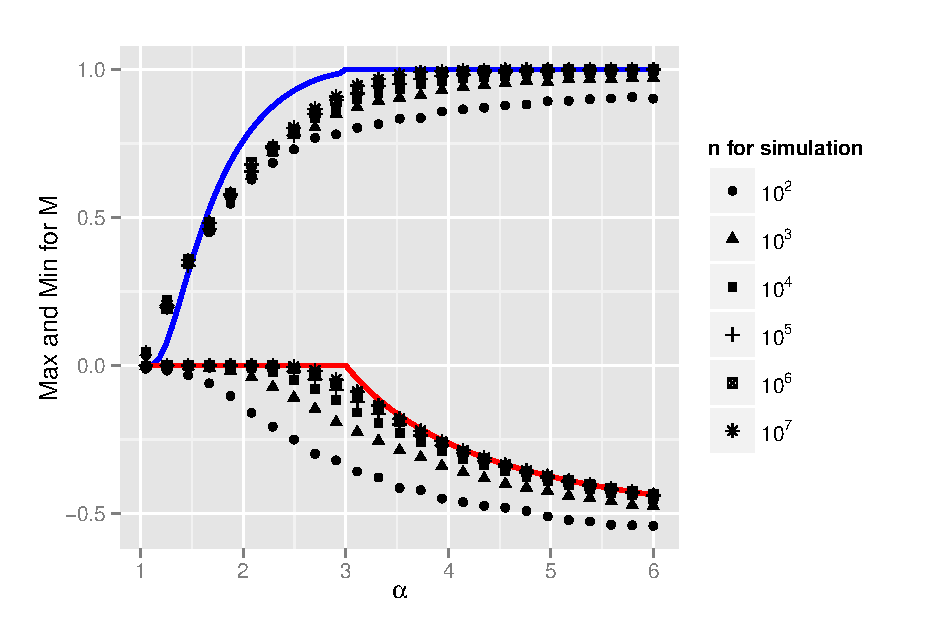
\includegraphics[width=0.9\columnwidth]{figures/ch3_limitedSysSizeEffect.eps}
\caption{Theoretical bounds for $ M_{\min} $ and $ M_{\max} $ and numerical simulations with different series lengths. Each point in simulation is produced by averaging 1000 independent runs.}
\label{fig:limitedSysSize}
\end{center}
\end{figure}
To summarize, as shown by the solid curves in Fig. \ref{fig:limitedSysSize}, when $ \alpha $ grows from 1 to 3, the lower bound remains 0 while the upper bounds increases from 0 to +1, constraining $ M $ to the positive region; when $ \alpha $ grows above 3, the upper bound remains +1 while the lower bound slides down to the negative region as a decreasing function of $ \alpha $, but with the limit $ M_{\min} \rightarrow -0.64 \ (\alpha \rightarrow \infty) $. Fig. \ref{fig:limitedSysSize} also reports the numerical values of $ M_{\min} $ and $ M_{\max} $ of series with finite lengths, produced by drawing independent samples and permuting them by $ \theta_{\min} $ and $ \theta_{\max} $. The gap resulted from finite system size diminishes with larger $ n $. 

\section{Empirical studies}
We study the distribution of memory against the scaling exponent from empirical time series data that follow power-law distributions. To this end, we use \textit{inter-event time series} data collected from online human activities. Inter-event time series refer to the series made up of time intervals between consecutive events and have been widely found to follow power-law distributions. 

The \textit{Movielens} dataset collects the time stamps for the users on its website\footnote{www.movielens.org} when they make a rating for movies. Then, one user corresponds to one inter-event time series, which is composed of time intervals between every two consecutive ratings. And the \textit{Twitter} dataset collects the time stamps when users send a tweet. Then the inter-event time series for a user is made up of time intervals between every two tweeting actions of him or her.

Because the datasets do not explicitly contain the parameters for power-law, we estimate the scaling exponent $ \alpha $ with the MLE method proposed by \cite{Clauset2009}. As we are examining the property of long power-law series, we rule out those series that are either too short ($ n<190 $)  or are unlikely to follow a power-law ($ p-value<0.1 $). $ p-value $ is used as a goodness-of-fit test based on the Kolmogorov-Smirnov (KS) statistic and likelihood ratios, which is also suggested by \cite{Clauset2009}.


\begin{figure}[!h]
\begin{center}
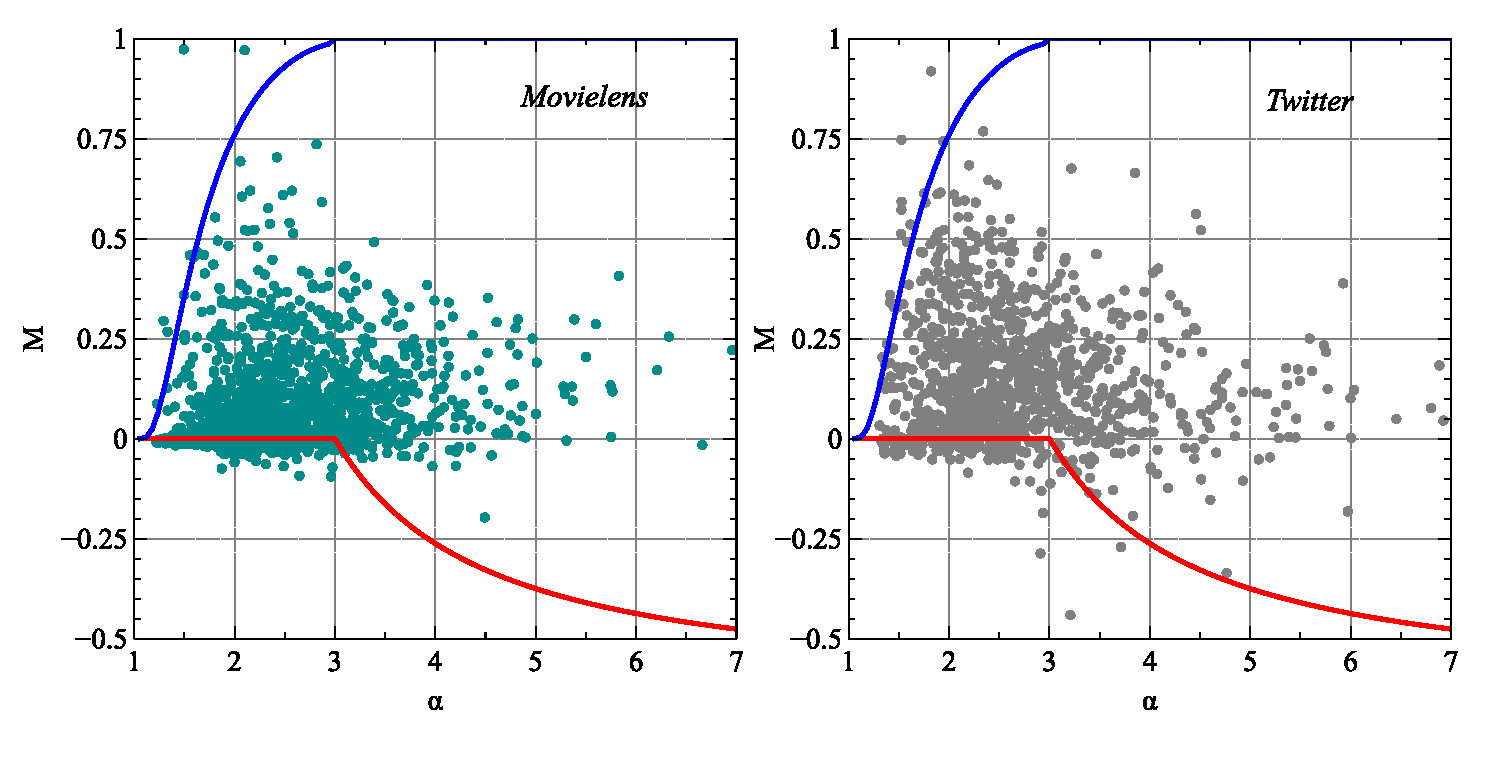
\includegraphics[width=0.95\textwidth]{figures/ch3_empirical_mem.eps}
\caption{Memory for power-law distributed inter-event time series from empirical inter-event time series, where each series is represented by a point and theoretical bounds are drawn as solid curves. The regions of memory from empirical data agree with theoretical bounds. Left: \textit{MovieLens} dataset for online movie rating. Right: \textit{Twitter} dataset for sending tweets. }
\label{fig:movlens}
\end{center}
\end{figure}
In agreement with theoretical values, we find the memory constraints existing in empirical power-law data. Fig. \ref{fig:movlens} plots $(\alpha, M)$ for power-law distributed inter-event time series selected from the \textit{MovieLens} dataset and the \textit{Twitter} dataset. Data points in both datasets fall into the regions predicted by theoretical bounds. A few outliers are either due to the last interval being exceptionally large (beyond the upper bounds) or the fact that they are programmed robots that perform actions at fixed times (beyond the lower bound).







% !TEX TS-program = xelatex
% !TEX root = Thesis_Guo2013.tex
% !Mode:: "TeX:UTF-8"

\chapter{Conclusion and Future Work}
\section{Summary of contributions}
The major methodological contribution of this work is the \textit{Equiprobable Partition Method} (EPM) presented in this thesis. We have showed that, in the convergent moment case, EPM is accurate when the number of partitions extends to infinity. And we have demonstrated that, in the divergent moment case, how EPM can be used as a method to effectively obtain the asymptotics of moments as a function of the sample size. Specifically, an EPM estimator for diverging sample moments consists two terms --- the leading order term characterizes the speed of polynomial divergence and the remaining term describes the details when the divergence is taken away. This is useful in treating statistics made up of several moments: by comparing the leading orders, we can preserve those with highest diverging orders only and neglecting others in large sample size; after canceling moments with the same leading order, we can learn the behavior of the $ \frac{\infty}{\infty} $-form statistics by referring to the remaining terms.   

As another major contribution of this thesis, we pointed out a special statistical property of power-law distributions that has not been presented before. With a permutational approach, by using both EPM for the divergent moment case and the traditional probabilistic method for the convergent moment case, we have derived the non-trivial bounds for the 1st-order autocorrelation (memory) of power-law series. The bounds are narrower than the natural bounds and are dependent on the power-law exponent, which suggests that the space for interdependence among series allowed by power-law is smaller than that allowed by Gaussian or uniform distributions and this effect is even related to the scaling exponent. This discovery also points out the risk of comparing the memory effect of different systems with the same quantity. Although this is a common practice, it might be unfair since the interdependence space allowed by different systems may be different. 

\section{Future work}
For the \textit{Equiprobable Partition Method}, we still need to prove the accuracy of EPM estimators for diverging sample moments, or to construct the bounds for the errors. Ideally, I feel this can be done by proving an asymptotic convergence property in parallel to what we have done for the convergent moment case. 

To be specific, supposing the EPM estimator for the diverging sample moment $ \mu_k' $ is $ n^{\gamma} g(n) $, we need to prove that, for any $ \epsilon>0 $, it holds that 

\begin{equation}
\lim_{n \rightarrow \infty} P \left ( \big | \frac{1}{n^{\gamma+1}} \sum_{i=1}^n x_i^k - g(n) \big | \geq \epsilon \right ) = 0.
\end{equation}

Another direction of future work would be a further analysis of the interdependence structure of the time series with heavy-tailed distributions. We need a deeper understanding for the interdependence structure beyond the simplest characterization given by the 1st-order autocorrelation, and for a wider family distributions more than power-law. Meanwhile, it would be useful to develop quantities for describing interdependence that does not cause marginal-specific bias. 







\end{document}

